\section{CONTROL DE CORRIENTE}
\label{sec:control_corriente}

\subsection{Objetivo y estado}
\label{sec:cc_objetivo}
El torque de un motor de corriente continua de imán permanente es proporcional a la corriente, $\tau_m = K_t\,i$. Para que la fuerza en el mando sea la que calculan los efectos, hay que imponer la corriente y no el ciclo de trabajo: con un ciclo de trabajo fijo, la corriente depende además de la resistencia, de la temperatura y de la velocidad a la que la mano mueve el eje (Sección~\ref{sec:motor775}).

Esta sección desarrolla el diseño de ese lazo de corriente: la conversión del comando en amperes, el cálculo del controlador según el apunte de la cátedra de Electrónica de Potencia \cite{oros2010}, su paso a tiempo discreto y su verificación en MATLAB y Simulink con el motor caracterizado en la Sección~\ref{sec:motor775}. El requisito principal es temporal: el lazo de efectos entrega un comando nuevo cada 2 ms, y la corriente debe alcanzar cada valor antes de que llegue el siguiente.

\textbf{Estado.} El diseño está calculado y simulado, pero no implementado en el firmware ni ensayado. El firmware actual aplica el comando directamente como ciclo de trabajo a 490 Hz. Los resultados de esta sección son, por lo tanto, de simulación, y se señalan como supuestos los valores que no provienen de una medición. Las corrientes máximas de cada eje son una propuesta a validar con la reductora.

\subsection{Origen de la información}
\label{sec:cc_fuentes}
\begin{center}
\begin{tabular}{p{0.34\textwidth}p{0.58\textwidth}}\toprule
Elemento & Origen\\\midrule
Estructura en cascada y regla de frecuencia de cruce & Apunte \cite{oros2010}, secc. 7.9.1, págs. 7.34--7.35\\
Modelo promediado del convertidor ($k_{PWM}$) & Apunte, secc. 7.9.1, ec. 7.54--7.55, págs. 7.35--7.36\\
Modelo del motor para el diseño & Apunte, secc. 7.9.2, ec. 7.56--7.61, págs. 7.36--7.37\\
Cálculo del PI de corriente & Apunte, secc. 7.9.4.1, ec. 7.67--7.71, págs. 7.39--7.40\\
Rizado de corriente con PWM unipolar & Apunte, secc. 7.8.5, ec. 7.51, pág. 7.34\\
Límites y anti-windup & Apunte, secc. 7.9.6 y 7.9.7, págs. 7.45--7.46; recálculo: \cite{astrom2020}, secc. 11.4\\
Márgenes, criterio de Nyquist y valores recomendados & \cite{astrom2020}, secc. 10.2 y 10.3, págs. 10-6 y 10-14 a 10-17\\
Estabilidad de sistemas discretos & \cite{astrom2008}, ejercicio del cap. 5, pág. 165\\
Lugar de raíces, márgenes sobre el Bode y digitalización & Temario de Sistemas de Control \cite{sistcontrol2025}\\
Funciones de MATLAB & \cite{mathworks_control}\\
Parámetros del motor & Mediciones propias (Subsección~\ref{sec:motor775_parametros})\\
Bloque \emph{Motor DC} de Simulink & \code{MotorModeloFFB.slx} (Subsección~\ref{sec:motor775_simulink})\\
Frecuencia máxima del driver & Hoja de datos del BTS7960 \cite{bts7960} y guía del módulo \cite{bts7960mod}, pág. 1: 25 kHz\\
Sensor de corriente y conversores & Hojas de datos del ACS712 \cite{acs712}, RP2350 \cite{rp2350} y ADS1115 \cite{ads1115}\\
Comando, período y límites & Código del firmware: \code{include/mis_defines.h}, \code{include/SimEffects.h} y \code{include/MotorDriver.h}\\\bottomrule
\end{tabular}
\end{center}

El apunte diseña en tiempo continuo, para un motor cuya velocidad impone la carga a través de la inercia. No trata el muestreo, el retardo de cálculo, la resolución del conversor ni un eje movido por la mano. Esos aspectos se agregan en las Subsecciones~\ref{sec:cc_discreto} a~\ref{sec:cc_resultados}. Al usarlo se encontró que la ec. 7.54 imprime la ganancia del convertidor invertida: lo correcto es $k_{PWM} = v_a/v_c = V_d/\hat V_{tri}$, valor con el que se obtienen los resultados del propio ejemplo.

\subsection{Del comando a la corriente}
\label{sec:cc_escala}
El lazo de efectos entrega un comando adimensional $u$ entre $-1$ y $+1$, que no tiene por sí mismo un significado en amperes. Se define una corriente de fondo de escala $I_{FS}$ para cada eje:
\begin{equation}
I^* = u\,I_{FS},\qquad \tau_{eje} = \eta\,N\,K_t\,I^*,
\label{eq:cc_escala}
\end{equation}
donde $I^*$ es la corriente de referencia [A], $N$ la relación de la reductora y $\eta$ su rendimiento, todavía no medido. Los valores que siguen son ideales ($\eta = 1$). El firmware limita el comando a $|u| \leq 220/255 = 0.863$ (\code{SIMCONNECT_EXTRA_LIMIT}), de modo que la corriente máxima pedida es $0.863\,I_{FS}$.

La elección de $I_{FS}$ está acotada por cuatro datos:
\begin{itemize}
\item \textbf{Corriente de rotor trabado.} Con el techo de PWM y 24 V, $0.863\cdot 24/0.869 = 23.8$ A. Es la corriente a la que tiende hoy el motor trabado con comando máximo, sin lazo. Supera el rango del ACS712 de 20 A y la capacidad de la fuente.
\item \textbf{Límite térmico.} La corriente continua admisible se estimó en 1.8 A sin ventilación (Subsección~\ref{sec:motor775_e6}). Los valores mayores solo pueden sostenerse un tiempo corto, por lo que el firmware deberá incluir un limitador $I^2t$.
\item \textbf{Rozamiento.} El motor despega con 0.39 A (Ensayo 5). Un comando menor que $0.39/I_{FS}$ no alcanza a moverlo: cuanto menor es $I_{FS}$, mayor es esa zona muerta.
\item \textbf{Reductora.} Multiplica el torque por $N$, pero también el rozamiento, y la inercia del motor por $N^2$.
\end{itemize}

\begin{center}
\begin{tabular}{lcc}\toprule
 & Roll & Pitch\\\midrule
Relación $N$ & 13.7 & 19.2 (polea de 75 mm de diámetro)\\
$I_{FS}$ propuesta (hipótesis) & 5 A & 4 A\\
Efecto por ampere & 0.308 N$\cdot$m/A & 11.5 N/A\\
Con $u = 1$ & 1.54 N$\cdot$m & 46 N\\
Con el máximo real, $u = 0.863$ & 1.33 N$\cdot$m (4.31 A) & 40 N (3.45 A)\\
Con 1.8 A & 0.55 N$\cdot$m & 21 N\\
Zona muerta por rozamiento del motor & 7.8\% & 9.8\%\\\bottomrule
\end{tabular}
\end{center}
En roll se reemplazó la relación prevista de 1:3.7 por 1:13.7. Con la primera, la corriente continua admisible daba solo 0.15 N$\cdot$m. Si el torque resulta excesivo, se reduce bajando $I_{FS}$ por software. El rozamiento y la inercia que se sienten al mover el mando, en cambio, no se reducen de ese modo. El motor de pitch todavía no se caracterizó y se calcula con los parámetros del de roll.

\subsection{Diseño del controlador PI}
\label{sec:cc_pi}
\subsubsection{Planta}
Se parte de la Ecuación~\eqref{eq:motor775_electrica}. La constante mecánica es unas 20 veces mayor que la eléctrica (Subsección~\ref{sec:motor775_modelo}), de modo que la fuerza contraelectromotriz se trata como una perturbación lenta y la planta se reduce a
\begin{equation}
G(s) = \frac{I(s)}{V(s)} = \frac{1/R}{1 + s\,\tau_e},\qquad \tau_e = \frac{L}{R} = \frac{0.50\ \text{mH}}{0.869\ \Omega} = 0.576\ \text{ms}.
\label{eq:cc_planta}
\end{equation}
Se usa la resistencia del circuito con el driver, porque es la que ve el controlador.

\subsubsection{Frecuencia de PWM}
El rizado de corriente del PWM unipolar es máximo con ciclo de trabajo 0.5 (ec. 7.51 del apunte):
\begin{equation}
\Delta I_{pp,\max} = \frac{V_d}{4\,L\,f_s} = \frac{24}{4\cdot 0.50\times10^{-3}\cdot 20\times10^{3}} = 0.60\ \text{A}.
\label{eq:cc_rizado}
\end{equation}
Se adopta $f_s = 20$ kHz, dentro del máximo de 25 kHz del BTS7960. Con los 490 Hz actuales, el período (2.04 ms) es 3.5 veces $\tau_e$ y más largo que el propio período del lazo de efectos: la corriente casi alcanza su valor final en cada pulso, y no es posible regularla.

\subsubsection{Cálculo de las ganancias}
El controlador es $C(s) = K_p + K_i/s$. Según las ec. 7.68 y 7.71 del apunte, el cero se ubica sobre el polo eléctrico y la ganancia fija la frecuencia de cruce $\omega_c$. Si la salida del controlador se expresa en volts y el ciclo de trabajo se obtiene dividiendo por la tensión de alimentación, $k_{PWM} = 1$ y
\begin{equation}
\frac{K_p}{K_i} = \tau_e,\qquad K_i = \frac{\omega_c R}{k_{PWM}} = \omega_c R,\qquad K_p = \omega_c L,\qquad C(s)\,G(s) = \frac{\omega_c}{s}.
\label{eq:cc_ganancias}
\end{equation}
El lazo cerrado ideal es de primer orden, con constante de tiempo $1/\omega_c$ y margen de fase de $90^\circ$. El apunte recomienda un cruce entre una y dos décadas por debajo de $f_s$, es decir, entre 200 y 2000 Hz. Con $f_c = 1$ kHz ($f_s/20$):
\[
K_p = 2\pi\cdot1000\cdot0.50\times10^{-3} = 3.14\ \text{V/A},\qquad
K_i = 2\pi\cdot1000\cdot0.8687 = 5458\ \text{V/(A}\cdot\text{s)}.
\]

\textbf{Validación del procedimiento.} Antes de aplicarlo al motor 775 se reprodujo en MATLAB el ejemplo numérico del apunte (Tabla 7.3, pág. 7.38: $R_a = 2\ \Omega$, $L_a = 5.2$ mH, $k_{PWM} = 12$, cruce en 1 kHz). Se obtuvo $k_{iI} = 1047.2$, $k_{pI} = 2.723$, cruce en 1000.0 Hz y margen de fase de $90.0^\circ$. El apunte (pág. 7.41) indica 1050.0 y 2.73.

\subsection{Controlador discreto}
\label{sec:cc_discreto}
\subsubsection{Margen de fase real}
El firmware medirá la corriente una vez por período ($T_s = 50\ \mu$s), calculará y aplicará la tensión en el período siguiente. La retención y ese retardo restan fase. En MATLAB se discretizó la planta con retención de orden cero (\code{c2d}), se agregó un período de retardo y se usó el PI con integración de Euler hacia adelante. La elección de $f_c$ surge de la siguiente comparación, lineal y sin saturación:

\begin{center}
\begin{tabular}{ccccc}\toprule
$f_c$ [Hz] & Margen de fase & Margen de ganancia & Establecimiento al 2\% & Sobrepico\\\midrule
300 & $80.8^\circ$ & 20.9 dB & 1.75 ms & 0.0\%\\
500 & $75.8^\circ$ & 16.4 dB & 0.95 ms & 0.3\%\\
800 & $68.4^\circ$ & 12.4 dB & 0.45 ms & 0.6\%\\
\textbf{1000} & $\mathbf{63.3^\circ}$ & \textbf{10.4 dB} & \textbf{0.45 ms} & \textbf{2.2\%}\\
1500 & $50.4^\circ$ & 6.9 dB & 0.55 ms & 20.2\%\\
2000 & $37.2^\circ$ & 4.4 dB & 0.80 ms & 45.0\%\\\bottomrule
\end{tabular}
\end{center}
Con 300 Hz, el establecimiento consume casi todo el intervalo de 2 ms. Por encima de 1 kHz el sobrepico crece y el tiempo ya no mejora. Se adopta 1 kHz.

\textbf{Lectura de la Figura~\ref{fig:cc_bode}.} La curva continua es el diseño del apunte: la magnitud cae 20 dB por década, cruza 0 dB en 1 kHz y la fase es constante en $-90^\circ$. La curva de trazos es el lazo discreto con el retardo de cálculo: su magnitud casi coincide, pero la fase cae con la frecuencia, hasta cruzar $-180^\circ$ cerca de 3.3 kHz. En el cruce (963 Hz) quedan $63.3^\circ$ de margen, en lugar de $90^\circ$.

\begin{figure}[H]
\centering
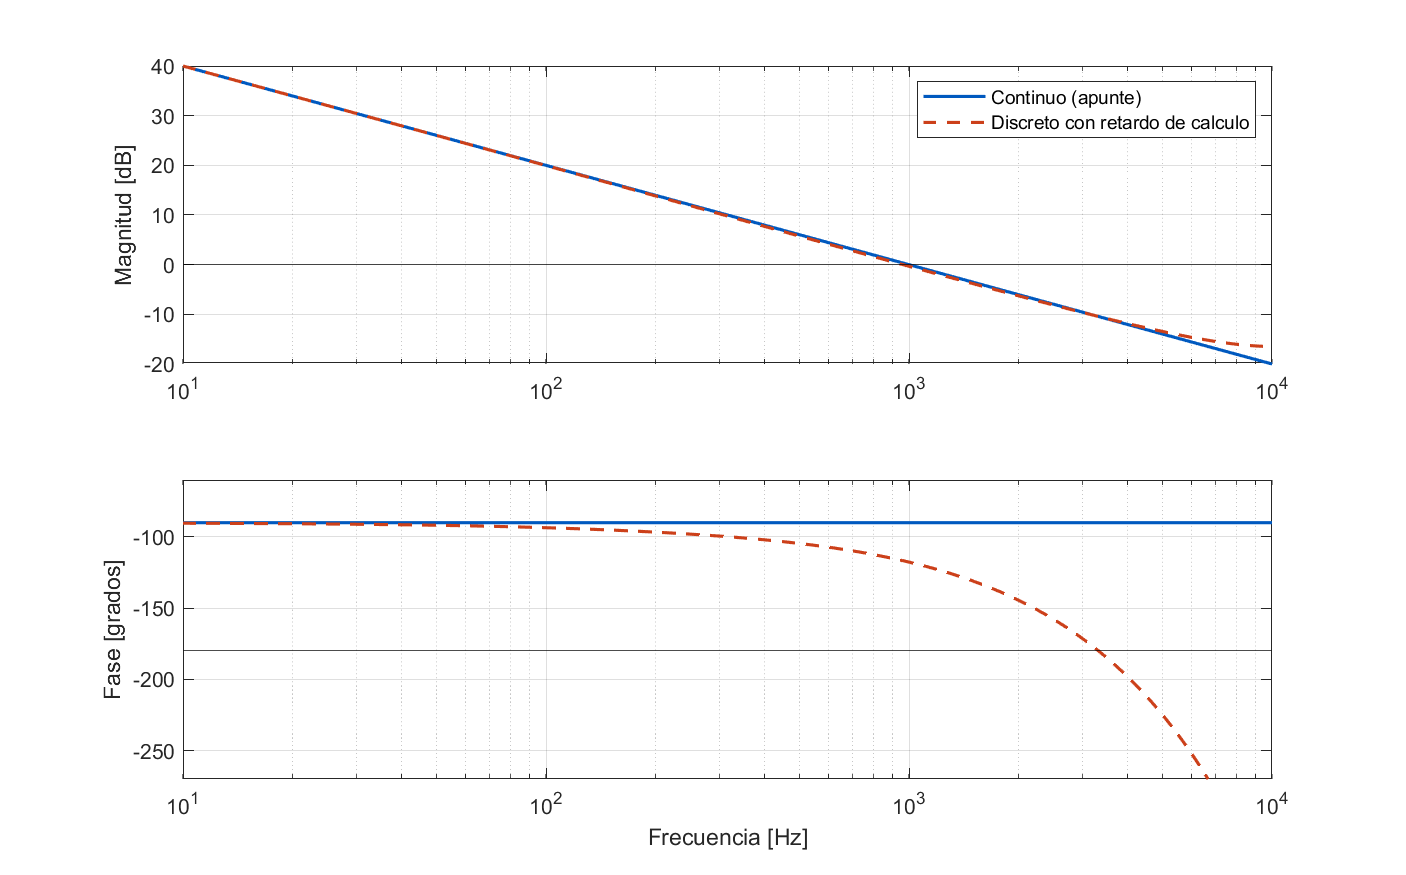
\includegraphics[width=0.85\textwidth]{figuras/control_corriente/bode.png}
\caption{Respuesta en frecuencia a lazo abierto del control de corriente de roll: diseño continuo y lazo discreto a 20 kHz con un período de retardo.}
\label{fig:cc_bode}
\end{figure}

\subsubsection{Algoritmo}
Con $e_k = I^*_k - i_k$, en cada período se calcula
\begin{align}
v_k &= K_p\,e_k + x_k, & v^{sat}_k &= \sat(v_k, \pm V_{max}),\nonumber\\
x_{k+1} &= x_k + K_i T_s\left[e_k + \frac{v^{sat}_k - v_k}{K_p}\right], & D_k &= \frac{v^{sat}_k}{V_{bus}},
\label{eq:cc_algoritmo}
\end{align}
donde $x$ es el estado del integrador, obtenido con la sustitución $s \to (z-1)/T_s$, una de las reglas de digitalización usadas en Sistemas de Control \cite{sistcontrol2025} (examen integrador, tema 4.3). La otra regla de la materia, la bilineal o de Tustin, $s \to \frac{2}{T_s}\frac{z-1}{z+1}$ (segundo parcial), da márgenes casi iguales, $62.9^\circ$ y 10.1 dB frente a $63.3^\circ$ y 10.4 dB. Se conserva la primera porque el integrador no depende del error del mismo período, lo que evita un lazo algebraico con el anti-windup. $x$ se expresa en volts, $V_{max} = (220/255)\,V_{bus} = 20.7$ V y $D$ el ciclo de trabajo con signo, que se aplica en el período siguiente.

\subsubsection{Anti-windup}
\label{sec:cc_aw}
En los saltos grandes, $K_p\,e$ supera la tensión disponible y la salida satura. El apunte propone congelar el integrador mientras la salida está saturada y el error empuja en el mismo sentido (secc. 7.9.7). La Ecuación~\eqref{eq:cc_algoritmo} usa en cambio el recálculo (\emph{back-calculation}) que presenta \cite{astrom2020} (secc. 11.4, Figura 11.11, págs. 11-16 y 11-17): una realimentación adicional lleva al integrador, con ganancia $k_{aw}$, la diferencia entre la salida aplicada y la pedida. Esa diferencia es nula sin saturación, de modo que no altera el diseño lineal. La referencia indica que $k_{aw}$ grande acorta el reinicio, que excesivo amplifica el ruido, y que una elección razonable es un múltiplo de la ganancia integral. Aquí $k_{aw} = K_i/K_p = 1/\tau_e = 1737\ \text{s}^{-1}$. Con esa elección, el integrador acumula solo el error que la tensión realmente aplicada pudo atender. Como el cero del PI coincide con el polo de la planta, eso evita la cola lenta, de constante $\tau_e$, que deja el congelamiento. En la simulación de referencia con comandos al azar e $I_{FS} = 10$ A, el error al final de los 2 ms fue de 0.15 A con congelamiento y 0.04 A con recálculo.

\textbf{Lectura de la Figura~\ref{fig:cc_aw}.} Ambas curvas coinciden mientras la tensión está saturada, porque la pendiente la fija la alimentación. Sin anti-windup, el integrador acumuló de más y la corriente llega a unos 11.4 A antes de volver a los 8.63 A pedidos. Con el recálculo, el sobrepico es de unos 0.3 A.

\begin{figure}[H]
\centering
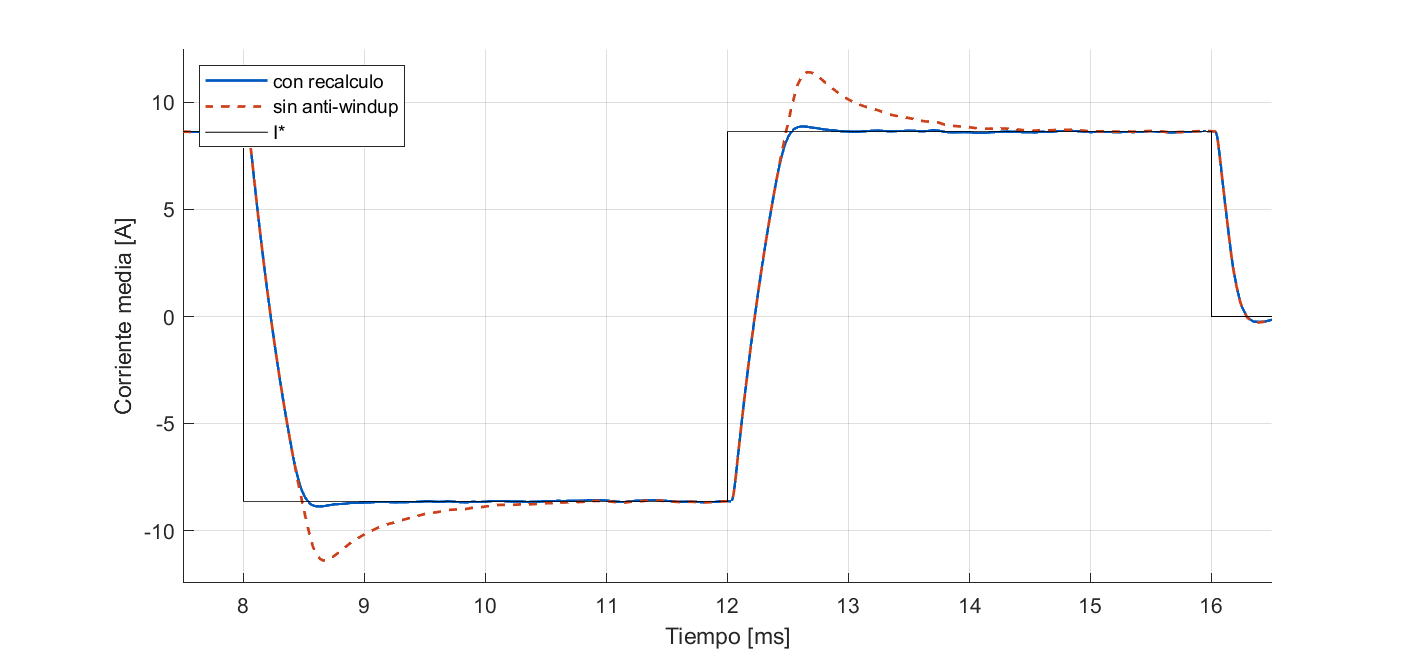
\includegraphics[width=0.85\textwidth]{figuras/control_corriente/antiwindup.png}
\caption{Efecto del anti-windup con saltos de $\pm 8.63$ A ($I_{FS} = 10$ A, para forzar la saturación): corriente media por período de PWM.}
\label{fig:cc_aw}
\end{figure}

\subsubsection{Prealimentaciones descartadas}
Se probaron dos términos adicionales. Sumar $R\,I^*$ es contraproducente: el PI ya cancela el polo eléctrico, y en la simulación con comandos al azar ($I_{FS}=5$ A) el sobrepico pasó de 0.18 a 1.40 A. Sumar $K_e\,\omega$ con la velocidad del encoder cada 2 ms no mejoró el resultado: con rotor libre, el error final fue 0.066 A, frente a 0.060 A sin él. El bloque queda en el modelo, desactivado.

\subsection{Estabilidad y márgenes}
\label{sec:cc_estabilidad}
\subsubsection{Criterios}
Sea $L(z) = C(z)\,z^{-1}G(z)$ la función de transferencia de lazo, con la planta discretizada y el retardo de cálculo. Se usan las siguientes medidas \cite{astrom2020} (secc. 10.3, págs. 10-14 a 10-17):
\begin{itemize}
\item \textbf{Margen de ganancia} $g_m = 1/|L(i\omega_{pc})|$: factor por el que puede aumentar la ganancia antes de la inestabilidad. $\omega_{pc}$ es la frecuencia en que la fase vale $-180^\circ$.
\item \textbf{Margen de fase} $\varphi_m = 180^\circ + \angle L(i\omega_{gc})$: atraso de fase adicional admisible. $\omega_{gc}$ es la frecuencia en que $|L| = 1$.
\item \textbf{Margen de estabilidad} $s_m$: menor distancia de la curva de Nyquist al punto crítico $-1$. Es el inverso del máximo de la sensibilidad, $M_s = \max|1/(1+L)| = 1/s_m$. Detecta casos en que los dos márgenes clásicos son buenos y, sin embargo, la curva pasa cerca de $-1$.
\item \textbf{Margen de retardo} $\varphi_m/\omega_{gc}$ (con $\varphi_m$ en radianes): retardo adicional que admite el lazo cuando hay un solo cruce de ganancia.
\end{itemize}
La referencia da como valores razonables $\varphi_m = 30^\circ$--$60^\circ$, $g_m = 2$--$5$ (6--14 dB) y $s_m = 0.5$--$0.8$ (pág. 10-17). La lectura de ambos márgenes sobre el diagrama de Bode es, además, parte del temario de Sistemas de Control \cite{sistcontrol2025} (segundo parcial, tema 2).

\subsubsection{Resultado del diseño}
\begin{center}
\begin{tabular}{lccl}\toprule
Medida & Nominal & Con el filtro del sensor & Valor razonable \cite{astrom2020}\\\midrule
Margen de fase & $63.3^\circ$ & $60.8^\circ$ & $30^\circ$--$60^\circ$\\
Margen de ganancia & 10.4 dB (3.32) & 10.2 dB (3.23) & 6--14 dB (2--5)\\
Margen de estabilidad $s_m$ & 0.65 & 0.63 & 0.5--0.8\\
Sensibilidad máxima $M_s$ & 1.53 & 1.58 & 1.25--2 ($1/s_m$)\\
Margen de retardo & 183 $\mu$s (3.7 períodos) & 176 $\mu$s & ---\\
Cruce de ganancia / de fase & 963 / 3326 Hz & 957 / 3036 Hz & ---\\\bottomrule
\end{tabular}
\end{center}
La segunda columna agrega el polo del divisor (6.1 $\mu$s) y el del ACS712 (80 kHz \cite{acs712}). Ambas cumplen los valores recomendados, y el margen de fase alcanza o supera levemente el extremo superior: se prefirió poco sobrepico. En la frecuencia de muestreo y el cruce elegidos, la pérdida de fase de un PI que cancela el polo se explica por el retardo equivalente de unas 1.5 muestras: $360^\circ\cdot 963\cdot 1.5\cdot 50\times10^{-6} = 26^\circ$, y quedarían $90^\circ - 26^\circ = 64^\circ$, de acuerdo con el valor calculado.

\textbf{Lectura de la Figura~\ref{fig:cc_margenes}.} El segmento del panel superior mide el margen de ganancia: en la frecuencia en que la fase llega a $-180^\circ$, la magnitud está 10.4 dB por debajo de 0 dB. El del panel inferior mide el margen de fase: en la frecuencia en que la magnitud cruza 0 dB, faltan $63.3^\circ$ para llegar a $-180^\circ$.

\begin{figure}[H]
\centering
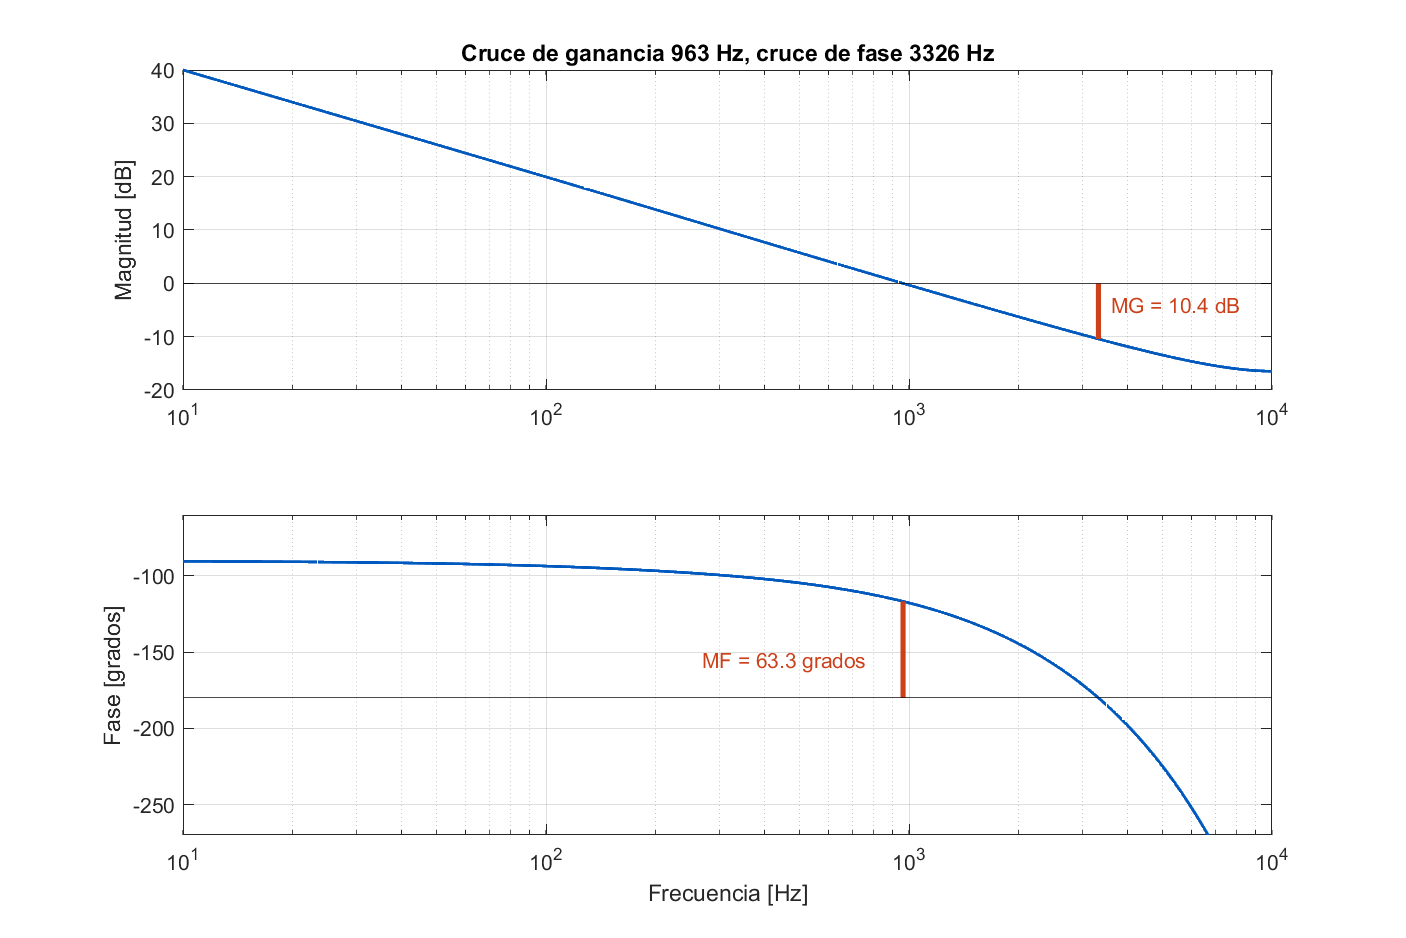
\includegraphics[width=0.85\textwidth]{figuras/control_corriente/margenes.png}
\caption{Margen de ganancia y margen de fase del lazo discreto nominal.}
\label{fig:cc_margenes}
\end{figure}

\textbf{Lectura de la Figura~\ref{fig:cc_nyquist}.} El lazo no tiene polos inestables (solo el integrador, en $z=1$, equivalente al origen). En ese caso, el lazo cerrado es estable si y solo si la curva no encierra el punto $-1$ (criterio de Nyquist simplificado, \cite{astrom2020}, Teorema 10.1, pág. 10-6; enunciado en tiempo continuo, se aplica aquí a la respuesta en frecuencia del lazo muestreado). La curva corta el eje real negativo en $-0.30$, es decir, $1/3.32$, a la derecha de $-1$: no lo encierra. El círculo en torno de $-1$, de radio $s_m = 0.65$, es tangente a la curva en su punto más cercano.

\begin{figure}[H]
\centering
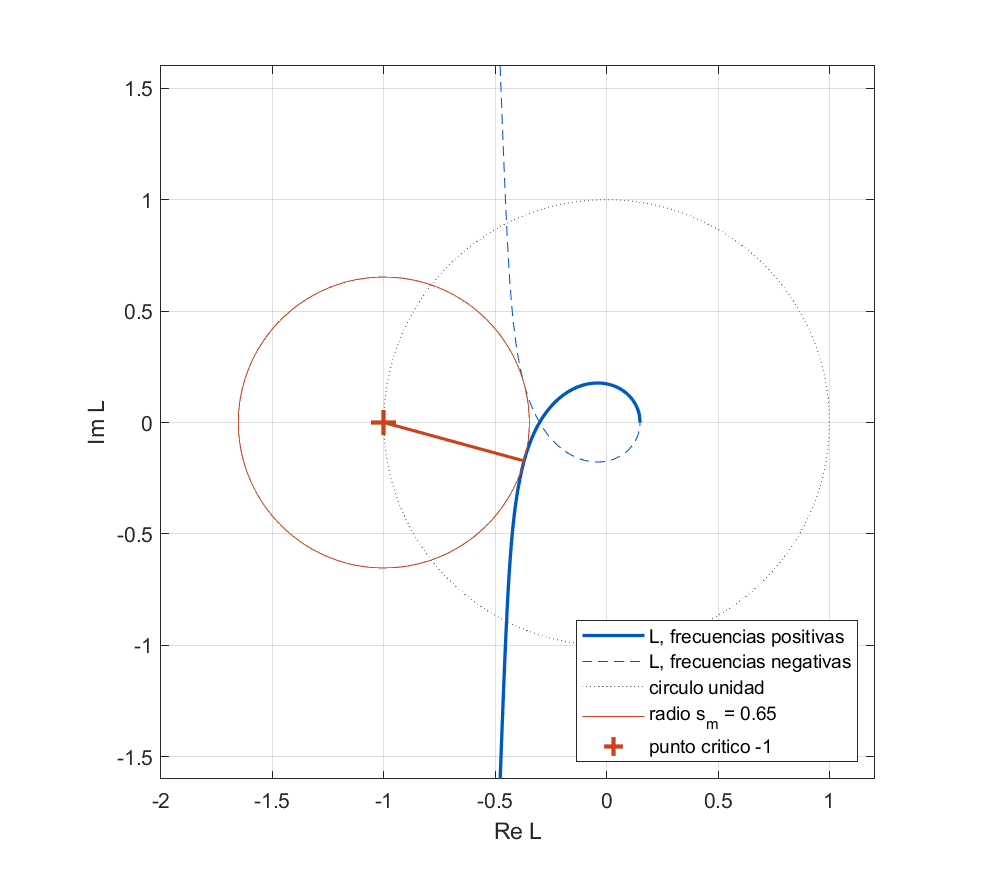
\includegraphics[width=0.6\textwidth]{figuras/control_corriente/nyquist.png}
\caption{Diagrama de Nyquist del lazo discreto nominal y margen de estabilidad $s_m$.}
\label{fig:cc_nyquist}
\end{figure}

\textbf{Lectura de la Figura~\ref{fig:cc_lgr}.} Un sistema discreto es asintóticamente estable si y solo si todos sus autovalores tienen módulo menor que 1 \cite{astrom2008} (pág. 165). Los polos de lazo cerrado del diseño son $0.9118$ y $0.5025 \pm 0.2210i$, de módulo 0.549: todos están dentro del círculo unidad. El primero está junto al cero del PI, $1 - T_s/\tau_e = 0.913$: proviene del polo eléctrico ($e^{-T_s/\tau_e} = 0.917$), casi cancelado, y no domina la respuesta a la referencia; sí aparece, lento, frente a perturbaciones o saturaciones, que es la razón del anti-windup de la Subsección~\ref{sec:cc_aw}. Al aumentar la ganancia, el par complejo se desplaza hacia el círculo y lo alcanza para $k = 3.32$, el mismo valor que el margen de ganancia.

\begin{figure}[H]
\centering
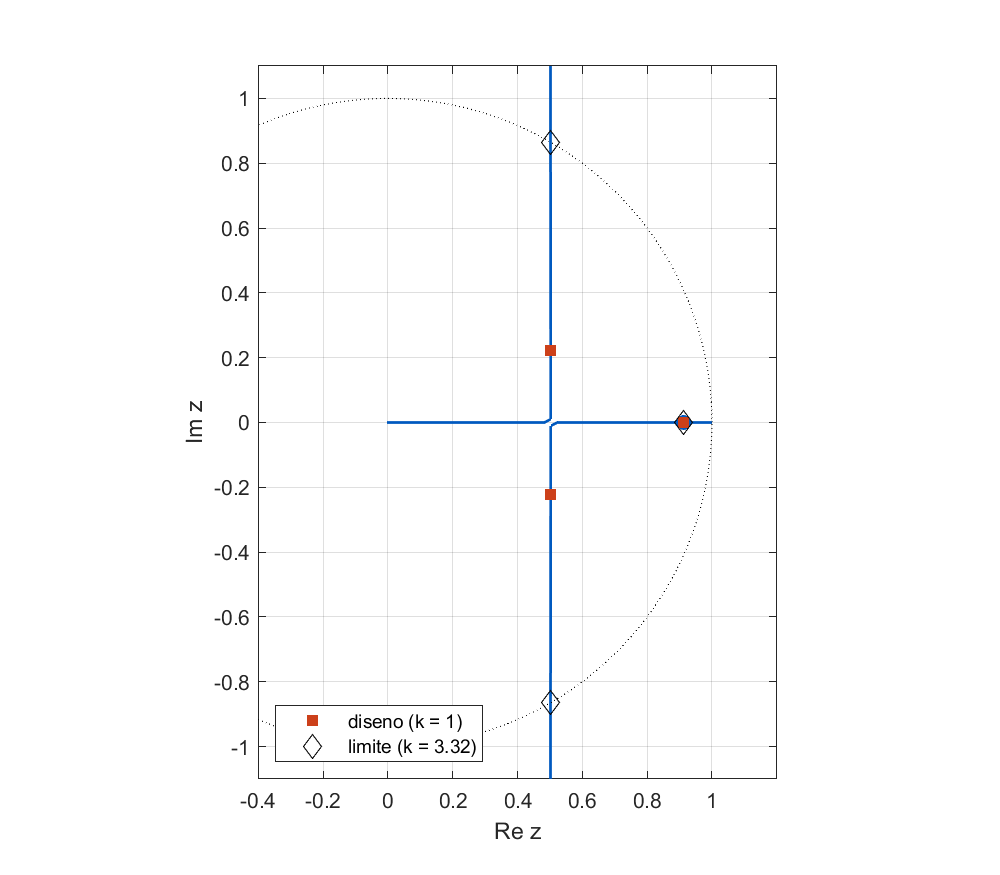
\includegraphics[width=0.6\textwidth]{figuras/control_corriente/lugar_raices.png}
\caption{Lugar de raíces en el plano $z$ al variar la ganancia del lazo.}
\label{fig:cc_lgr}
\end{figure}

\subsubsection{Error en régimen}
El lazo tiene un integrador: es de tipo 1. Según la clasificación por constantes de error \cite{sistcontrol2025} (primer parcial, tema 1), sigue un escalón sin error y una rampa con error constante. Por eso la corriente alcanza exactamente cada referencia, que es constante durante 2 ms. La fuerza contraelectromotriz actúa como perturbación: si crece como una rampa de pendiente $\dot e_a$, el error es $\dot e_a/K_i$, de 1.8 mA para 10 V/s.

\subsubsection{Robustez}
Los parámetros reales difieren de los nominales. La tabla recalcula los márgenes manteniendo las ganancias y el filtro del sensor, y cambiando la planta. Los valores de $R$ cubren el calentamiento y la resistencia del motor solo (0.66 $\Omega$); los de $L$ y $V_{bus}$, variaciones supuestas.
\begin{center}
\begin{tabular}{lcccc}\toprule
Caso & Margen de fase & Margen de ganancia & $s_m$ & Margen de retardo\\\midrule
Nominal & $60.8^\circ$ & 10.2 dB & 0.63 & 176 $\mu$s\\
$R$ +30\% & $66.1^\circ$ & 10.4 dB & 0.65 & 197 $\mu$s\\
$R = 0.66\ \Omega$ & $56.7^\circ$ & 10.1 dB & 0.62 & 162 $\mu$s\\
$L$ +30\% & $62.2^\circ$ & 12.4 dB & 0.70 & 228 $\mu$s\\
$L$ $-30$\% & $54.5^\circ$ & 7.4 dB & 0.52 & 114 $\mu$s\\
$L$ $-30$\% y $R$ +30\% & $60.4^\circ$ & 7.6 dB & 0.54 & 130 $\mu$s\\
$V_{bus}$ +10\% & $58.0^\circ$ & 9.4 dB & 0.60 & 153 $\mu$s\\
$V_{bus}$ $-10$\% & $63.5^\circ$ & 11.1 dB & 0.67 & 205 $\mu$s\\\bottomrule
\end{tabular}
\end{center}
El caso más desfavorable es una inductancia 30\% menor, y aun así cumple los valores recomendados. La inductancia medida varía con la frecuencia: 0.656 mH a 1 kHz, 0.50 mH a 10 kHz y un mínimo de 0.464 mH entre posiciones. El ensayo de $-30\%$ (0.35 mH) es más exigente que ese mínimo.

Los márgenes también justifican la elección de $f_c$: con 1500 Hz se obtienen $50.4^\circ$, 6.9 dB y $s_m = 0.50$, en el límite recomendado sin dejar reserva para esas variaciones; con 2000 Hz, $37.2^\circ$, 4.4 dB y $s_m = 0.36$, fuera de los valores recomendados.

\subsubsection{Comprobación en Simulink}
El margen de ganancia es una predicción verificable. En el modelo, con tensión promediada, el filtro del sensor, sin ruido y con un escalón pequeño (0.3 A) que no satura al comienzo, se multiplicaron $K_p$ y $K_i$ por un mismo factor. El límite calculado para ese caso es 3.28.

\textbf{Lectura de la Figura~\ref{fig:cc_margen_sim}.} Con el diseño ($\times 1$) la respuesta es rápida y casi sin sobrepico. Con $\times 2$ oscila y se amortigua. Con $\times 3$, debajo del límite, la oscilación decrece despacio. Con $\times 3.5$, encima del límite, crece hasta que la saturación la limita. La simulación confirma que el límite está entre 3 y 3.5.

\begin{figure}[H]
\centering
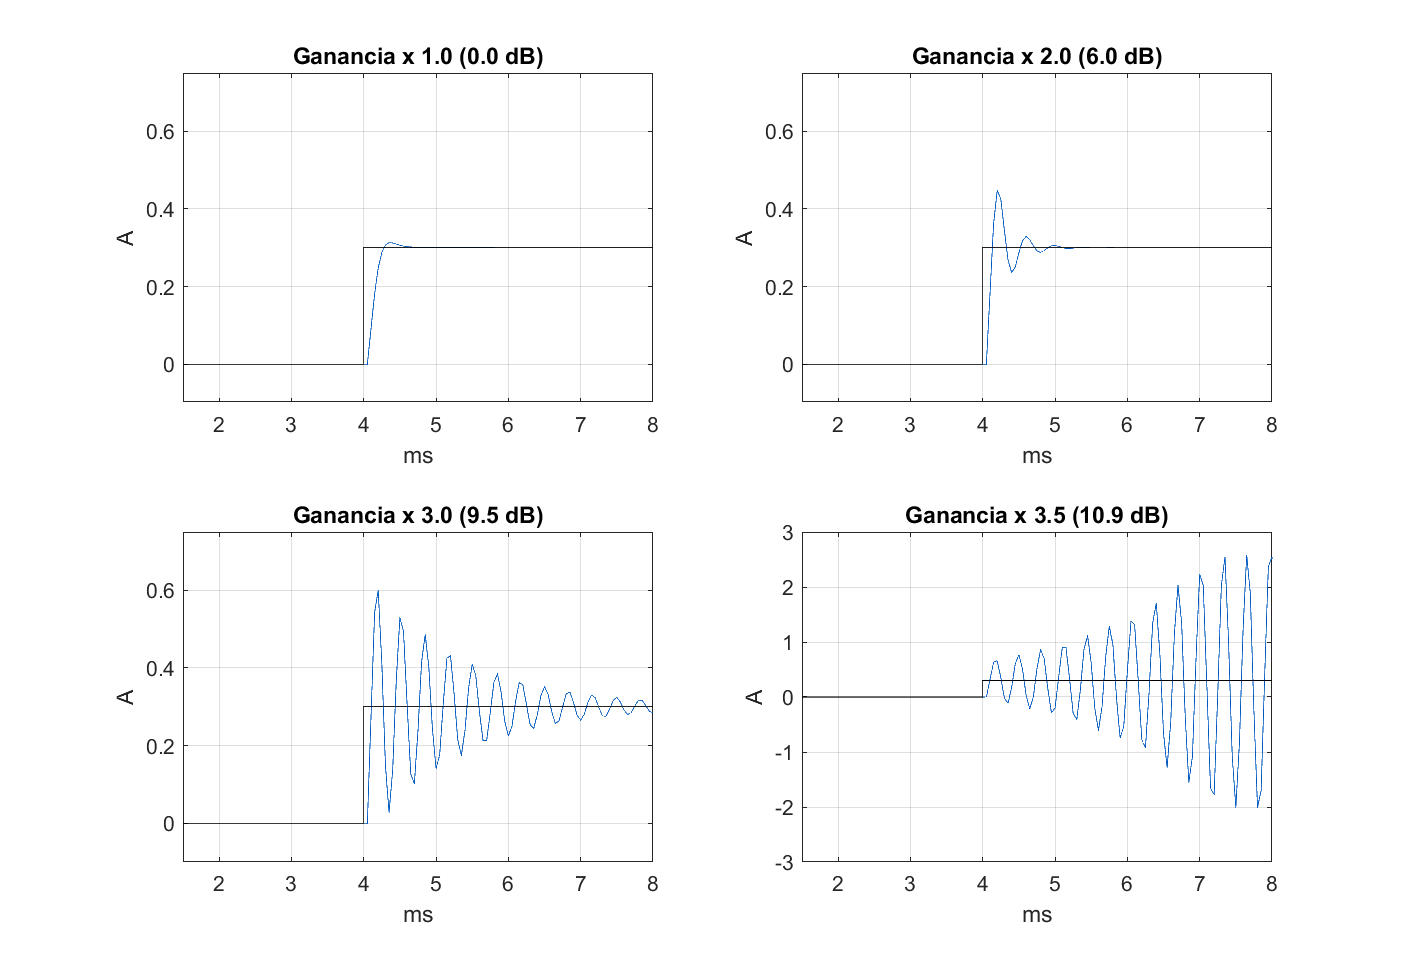
\includegraphics[width=0.85\textwidth]{figuras/control_corriente/margen_simulink.png}
\caption{Comprobación del margen de ganancia: escalón de 0.3 A con la ganancia multiplicada por 1, 2, 3 y 3.5 (la última, con otra escala).}
\label{fig:cc_margen_sim}
\end{figure}

\textbf{Alcance.} Estos márgenes son los del modelo lineal. No cubren la saturación (tratada con el anti-windup y las simulaciones de la Subsección~\ref{sec:cc_resultados}) ni la dinámica real del driver. Una estimación experimental, con un escalón o un barrido de frecuencia, forma parte de los próximos pasos.

\subsection{Medición de la corriente}
\label{sec:cc_medicion}
El lazo necesita una muestra por período de PWM. El ADS1115, previsto inicialmente, entrega 860 muestras por segundo como máximo \cite{ads1115} (pág. 1), unas 430 por eje al alternar dos canales: menos de una por cada comando de 2 ms. El conversor interno del RP2350 (12 bits, 9.2 bits efectivos y 500 kmuestras/s \cite{rp2350}, secc. 12.4) permite tomarlas sincronizadas con el PWM.

\textbf{Lectura de la Figura~\ref{fig:cc_ads}.} Los dos paneles superiores muestran el lazo propuesto, calculado con un script independiente del modelo de Simulink. El inferior muestra los mismos comandos con el ADS1115, prealimentación $R\,I^*$ y una corrección integral lenta, con una resistencia real 15\% mayor que la nominal. La corriente no alcanza la referencia: al final de los 2 ms queda un error de hasta 1.05 A, frente a 0.05 A del lazo propuesto.

\begin{figure}[H]
\centering
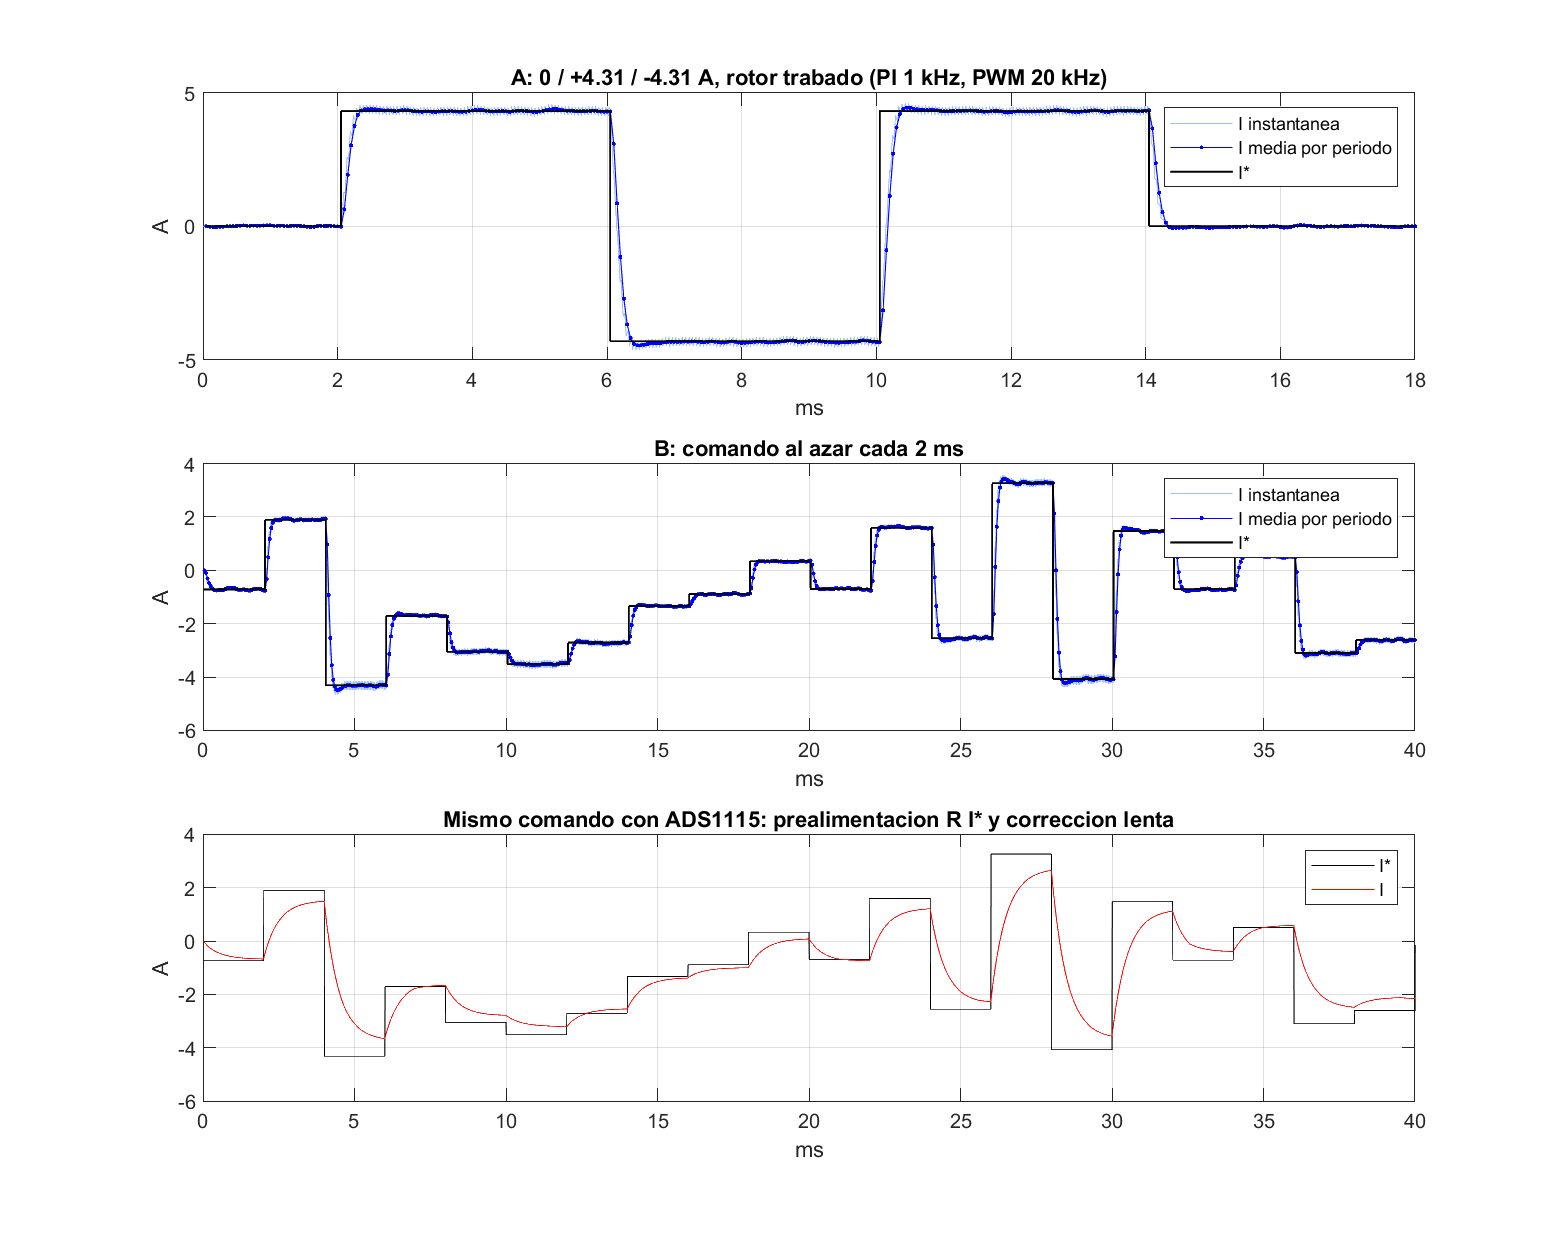
\includegraphics[width=0.85\textwidth]{figuras/control_corriente/ads1115.png}
\caption{Lazo con el conversor interno (arriba y centro) y con el ADS1115 (abajo), rotor trabado, $I_{FS} = 5$ A (script \code{Control_Corriente_775.m}).}
\label{fig:cc_ads}
\end{figure}

El ACS712 de 20 A entrega 2.5 V $\pm$ 0.1 V/A con alimentación de 5 V \cite{acs712}, y los pines analógicos del RP2350 admiten 3.3 V. Se adapta con un divisor de 4.7 k$\Omega$ y 6.8 k$\Omega$ (factor 0.591) y un capacitor de 2.2 nF junto al pin. La resistencia total, de 11.5 k$\Omega$, respeta la carga mínima de 4.7 k$\Omega$ del sensor. Un traductor de niveles digital, como el TXS0108E, no es aplicable: contiene circuitos que aceleran los flancos \cite{txs0108e} (secc. de descripción, págs. 16--17) y deformarían una señal analógica.

\textbf{Ruido.} El divisor atenúa por igual la señal y el ruido del sensor, y su ruido térmico equivale a unos 0.04 mA. Solo aumenta el efecto del conversor: el escalón de 12 bits pasa de 8 a 14 mA. Con 0.05 A eficaces supuestos para el sensor y los 9.2 bits efectivos del conversor, el ruido total pasa de 0.053 a 0.057 A (8\%). El valor supuesto se compara con la hoja de datos del ACS712 de 20 A, que indica 11 mV pico a pico típicos con 2 kHz de ancho de banda \cite{acs712}. Dividiendo por 6.6, son 0.017 A eficaces. Si el ruido fuera blanco, con el filtro del divisor (26 kHz) ascendería a unos 0.06 A, por el cociente de anchos de banda. La estimación es del mismo orden y debe verificarse con mediciones sin corriente. En el modelo promediado, 0.05, 0.10 y 0.20 A de ruido en la medición producen 0.023, 0.047 y 0.093 A eficaces en el motor: el lazo transmite algo menos de la mitad. Más importante es la alimentación: el sensor es ratiométrico \cite{acs712}, y una caída de 100 mV en los 5 V desplaza el cero 50 mV, equivalentes a 0.5 A. Por eso se prevé medir también los 5 V y calibrar el cero al encender.

\textbf{Instante de muestreo.} El RP2350 dispone de un modo de PWM de fase correcta, que centra el pulso sin importar el ciclo de trabajo, y genera una interrupción por período \cite{rp2350} (cap. 12, PWM). Con PWM centrado y rizado triangular, la corriente instantánea en el centro del intervalo de apagado coincide con su valor medio. El filtro del divisor ($\tau = 6.1\ \mu$s) retrasa el rizado, y la muestra deja de coincidir con la media. En Simulink, a 4.3 A y sin ruido, el sesgo es de $-0.038$ A si se muestrea en el centro, y de $+0.004$ A si se muestrea 6.1 $\mu$s después. Este desfase forma parte del diseño.

\subsection{Modelo de Simulink}
\label{sec:cc_simulink}
El modelo \code{Control_Corriente_FFB.slx} (carpeta \code{modelizacion motor 775/Control_Corriente}) toma una copia del subsistema \emph{Motor DC} validado en la Subsección~\ref{sec:motor775_validacion} y cierra el lazo a su alrededor. \code{MotorModeloFFB.slx} no se modificó. El modelo se genera con el script \code{Crear_Modelo_Control.m}, de modo que la construcción es reproducible.

\textbf{Lectura de la Figura~\ref{fig:cc_modelo}.} La señal recorre el diagrama de izquierda a derecha y vuelve por el sensor. La tabla siguiente explica cada bloque, su parámetro y el motivo por el que está.

\begin{longtable}{p{0.17\textwidth}p{0.21\textwidth}p{0.52\textwidth}}
\toprule Bloque & Parámetro & Qué hace y por qué\\\midrule\endhead
\emph{Comando +-1} & \code{cmd_ws}, período \code{Ts_cmd} = 2 ms & Entrega un valor entre $-1$ y $+1$ cada 2 ms y lo mantiene. Reproduce la salida del lazo de efectos del firmware (\code{CONTROL_LOOP_MS}).\\
\emph{Recorte} & \code{cmd_max} = 0.863 & Limita el comando como \code{SIMCONNECT_EXTRA_LIMIT}. Es el límite en la referencia que recomienda el apunte \cite{oros2010} (secc. 7.9.6).\\
\emph{I\_FS} & 5 A (roll) & Convierte el comando en corriente de referencia, Ecuación~\eqref{eq:cc_escala}.\\
\emph{2 ms a Ts} & \code{Ts} = 50 $\mu$s & Pasa la referencia del lazo de 2 ms al de 50 $\mu$s: el de corriente se ejecuta 40 veces por comando. Es la separación de velocidades de la cascada (secc. 7.9.1).\\
\emph{Error} & --- & Resta la corriente medida: es la realimentación negativa.\\
\emph{PI corriente} & \code{Kp}, \code{Ki} & Calcula la tensión necesaria (secc. 7.9.4.1). Se detalla más abajo.\\
\emph{Retardo calculo} & $1/z$, \code{Ts} & La tensión calculada se aplica en el período siguiente. Resta fase y define los márgenes de la Subsección~\ref{sec:cc_estabilidad}.\\
\emph{BTS7960 PWM} & \code{Vbus}, \code{usar_conmutado} & Convierte la tensión pedida en pulsos de 0 a $\pm 24$ V, o en su valor medio.\\
\emph{Motor DC} & $R$, $L$, $K_e$, $J$, $B$, $\tau_c$ & Planta, con parámetros medidos. Entradas: tensión, $T_L$ y $J_L$. Salidas: corriente, velocidad y posición.\\
\emph{Sensor ACS712 + ADC} & \code{k_acs}, \code{k_div}, \code{ruido_A} & Mide la corriente con sus imperfecciones y cierra el lazo.\\
\emph{Kt}, \emph{Reductora N} & 0.0225; 13.7 & Torque ideal en el eje. No intervienen en el lazo.\\
\emph{Encoder 2 ms}, \emph{w a Ts}, \emph{Ka (FCEM)} & \code{usar_FCEM} = 0 & Prealimentación de la fuerza contraelectromotriz con la velocidad muestreada. Es la idea del control anticipativo (secc. 7.9.5). Desactivada, porque no mejoró.\\
\emph{T\_L en el eje}, \emph{1 sobre N} & \code{tl_ws} & Torque externo en el eje de salida (la mano), referido al motor.\\
\emph{J\_L reflejada} & \code{J_eje}/$N^2$ & Inercia de reductora y mando, referida al motor.\\
\emph{Scope control} y salidas & --- & Gráficos y variables \code{I_ref}, \code{I_real}, \code{I_adc}, \code{V_motor}, \code{w_motor}, \code{T_eje} y \code{theta_motor}. No afectan la simulación.\\\bottomrule
\end{longtable}

\begin{figure}[H]
\centering
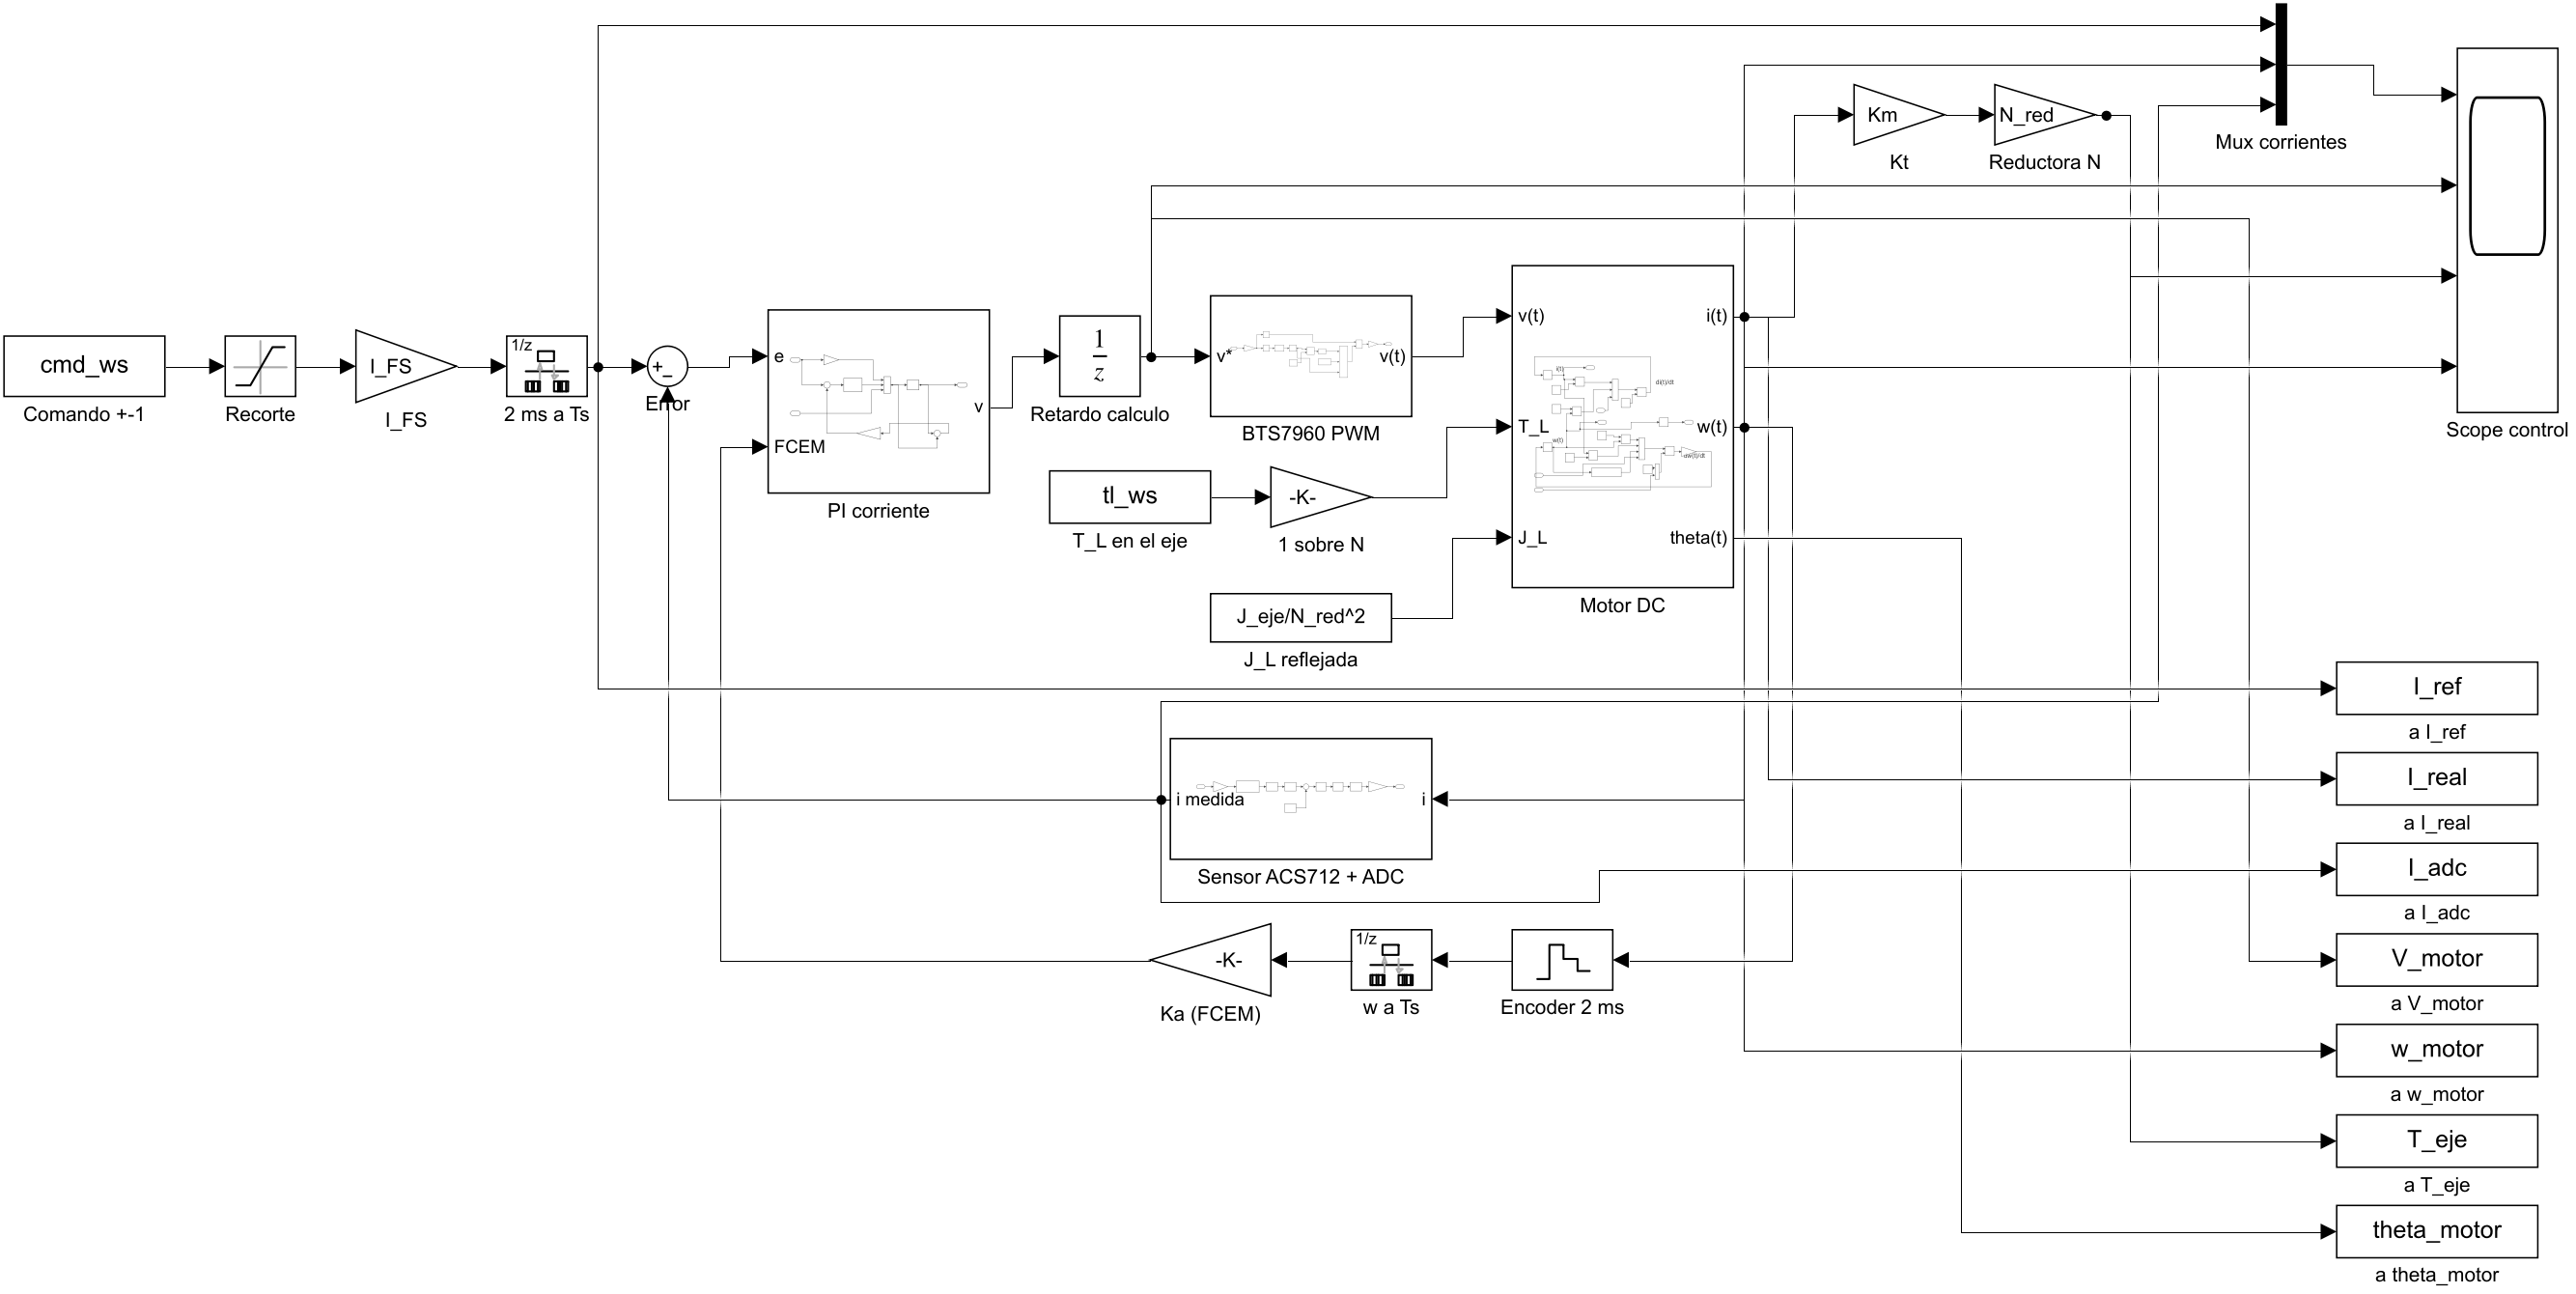
\includegraphics[width=\textwidth]{figuras/control_corriente/simulink_modelo.png}
\caption{Modelo \code{Control_Corriente_FFB.slx}: lazo de corriente alrededor del motor caracterizado.}
\label{fig:cc_modelo}
\end{figure}

\textbf{Lectura de la Figura~\ref{fig:cc_sim_pi}.} Es la Ecuación~\eqref{eq:cc_algoritmo}:
\begin{itemize}
\item \emph{Kp}: acción proporcional, reacciona al error del período actual.
\item \emph{Suma aw} e \emph{Integral Ki}: acción integral (Euler hacia adelante, $K_iT_s/(z-1)$). Acumula el error hasta anularlo y hace que el lazo sea de tipo 1.
\item \emph{Suma PI}: suma la parte proporcional, la integral y la prealimentación.
\item \emph{Limite Vmax}: recorta la salida a $\pm 20.7$ V, el techo de PWM del firmware. Representa el límite del convertidor (\cite{oros2010}, secc. 7.9.6 y Fig. 7.52).
\item \emph{vsat - v} y \emph{1 sobre Kp}: realimentan al integrador la tensión que no pudo aplicarse. Es el anti-windup (\cite{astrom2020}, Figura 11.11).
\end{itemize}

\begin{figure}[H]
\centering
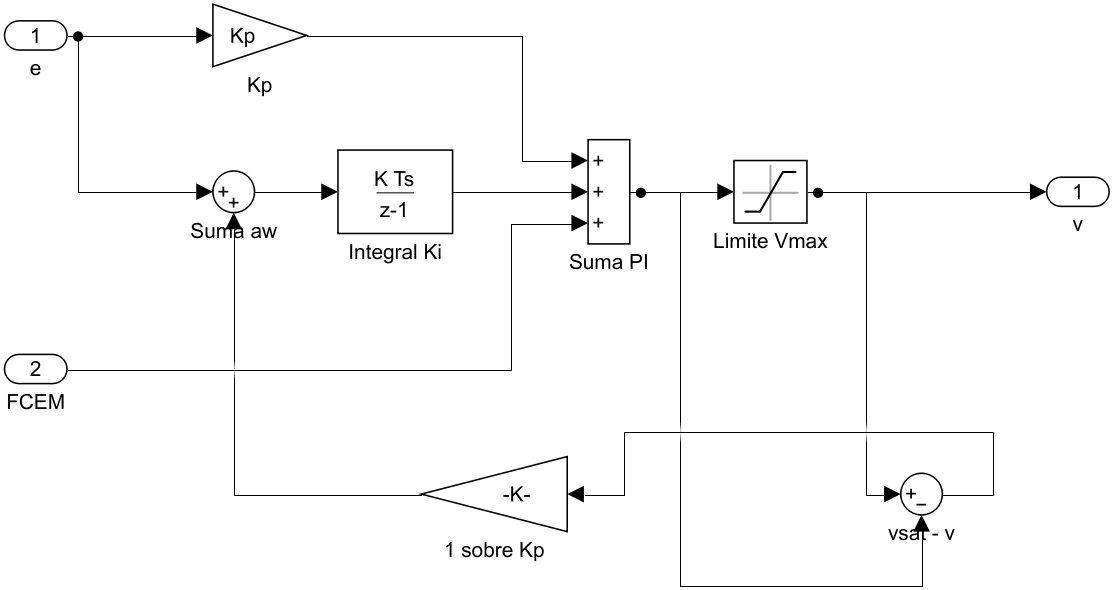
\includegraphics[width=0.7\textwidth]{figuras/control_corriente/simulink_pi.png}
\caption{Subsistema \emph{PI corriente}.}
\label{fig:cc_sim_pi}
\end{figure}

\textbf{Lectura de la Figura~\ref{fig:cc_sim_pwm}.} La señal recorre los bloques en este orden:
\begin{itemize}
\item \emph{1 sobre Vbus}: de volts a ciclo de trabajo. Compensa la ganancia del convertidor, y por eso $k_{PWM} = 1$.
\item \emph{Signo} y \emph{Abs}: separan el sentido, que elige la rama del puente que conmuta, y el módulo. Es el manejo unipolar (\cite{oros2010}, secc. 7.8.3), igual al de \code{MotorDriver.h}.
\item \emph{Pulso perdido}: resta un tiempo por período en que el driver no conduce. Vale cero hasta medirlo.
\item \emph{D 0..1}: limita el ciclo de trabajo.
\item \emph{Portadora} y \emph{Comparador}: triangular de 20 kHz; mientras el ciclo de trabajo la supera, hay pulso. Está desfasada 6.1 $\mu$s por el filtro del sensor (Subsección~\ref{sec:cc_medicion}).
\item \emph{a double}, \emph{conmutado} y \emph{Elegir}: seleccionan PWM conmutado o tensión promediada, que es el modelo lineal del apunte (secc. 7.9.1).
\item \emph{Prod} y \emph{Vbus}: devuelven el signo y llevan el resultado a $\pm 24$ V.
\end{itemize}

\begin{figure}[H]
\centering
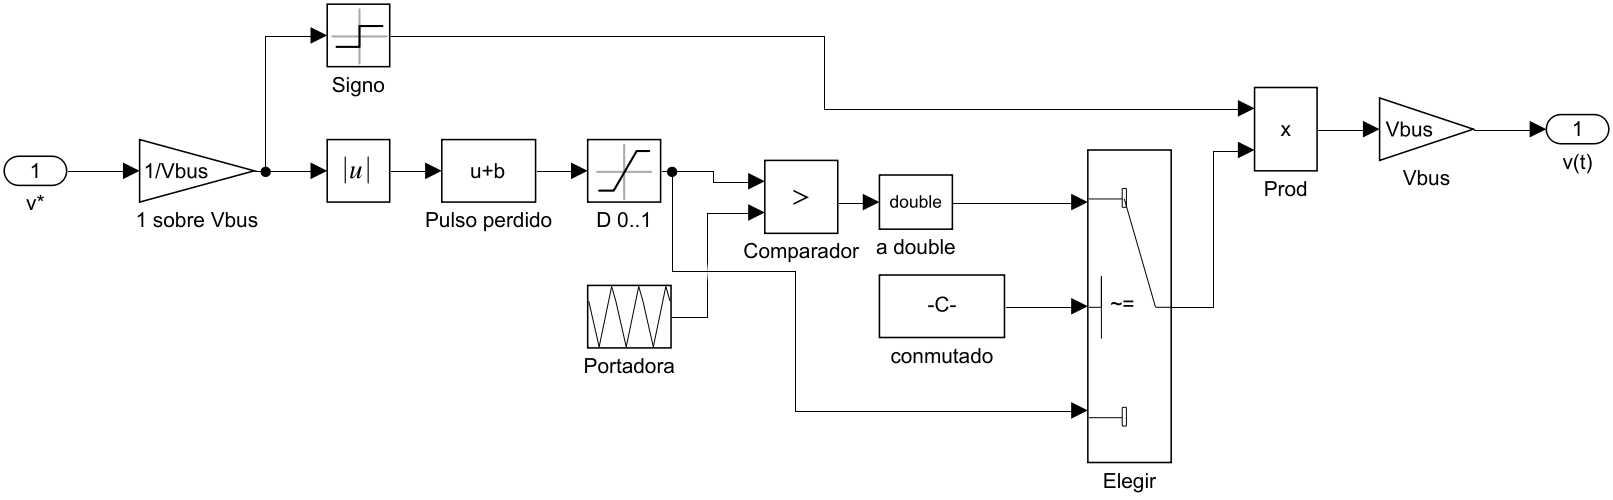
\includegraphics[width=0.85\textwidth]{figuras/control_corriente/simulink_pwm.png}
\caption{Subsistema \emph{BTS7960 PWM}: modulación unipolar centrada o tensión promediada.}
\label{fig:cc_sim_pwm}
\end{figure}

\textbf{Lectura de la Figura~\ref{fig:cc_sim_sensor}.} La señal recorre los bloques en este orden:
\begin{itemize}
\item \emph{ACS712 0.1 V por A}: sensibilidad de la versión de 20 A, 100 mV/A (\cite{acs712}).
\item \emph{Divisor 4.7k 6.8k 2.2nF}: atenuación de 0.591 y filtro de primer orden de 6.1 $\mu$s.
\item \emph{Cero}: suma la mitad de la alimentación, 2.5 V, ya atenuada. Está después del filtro para que la simulación arranque en régimen.
\item \emph{Muestreo}: una muestra cada 50 $\mu$s.
\item \emph{Ruido} y \emph{Suma}: ruido gaussiano, supuesto.
\item \emph{Rango 0-3.3 V} y \emph{ADC 12 bits}: saturación y escalones de 0.81 mV del conversor (\cite{rp2350}, secc. 12.4).
\item \emph{Resta cero} y \emph{a amperes}: conversión inversa, la que hará el firmware.
\end{itemize}

\begin{figure}[H]
\centering
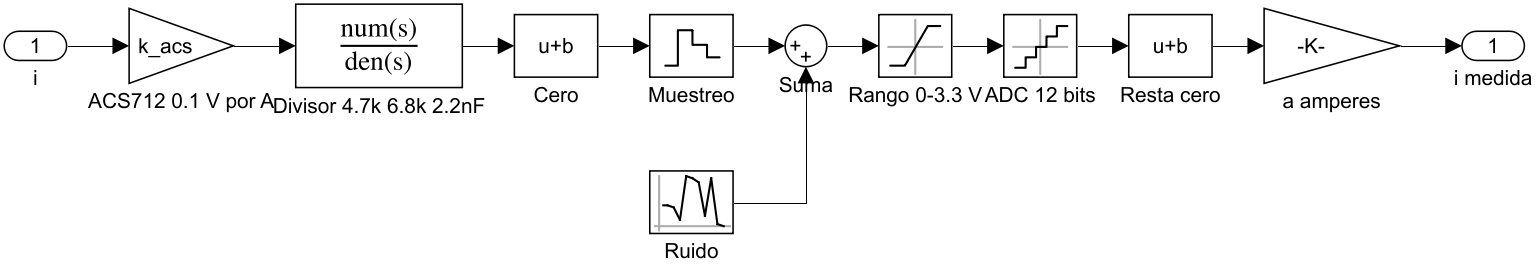
\includegraphics[width=0.95\textwidth]{figuras/control_corriente/simulink_sensor.png}
\caption{Subsistema \emph{Sensor ACS712 + ADC}.}
\label{fig:cc_sim_sensor}
\end{figure}

\textbf{Lectura de la Figura~\ref{fig:cc_sim_motor}.} Es el subsistema de la Figura~\ref{fig:motor775_simulink_motor} con dos entradas más. La parte superior resuelve la ecuación eléctrica: la suma calcula $v - R\,i - K_a\,\omega$, \emph{Divide} la divide por $L$ y el integrador entrega $i$. La inferior resuelve la mecánica: $K_m\,i - B\,\omega$ menos la \emph{Friccion seca}, dividido por la inercia e integrado, entrega $\omega$. \emph{Eje libre} anula la aceleración si el rotor está trabado y el último integrador entrega la posición. En las entradas agregadas, $T_L$ se resta en la suma de torques y $J_L$ se suma a $J$ antes de dividir:
\begin{equation}
(J + J_L)\,\frac{d\omega}{dt} = K_t\,i - B\,\omega - \tau_c\tanh\!\left(\frac{\omega}{\omega_{tc}}\right) - T_L,\qquad J_L = \frac{J_{eje}}{N^2},\quad T_L = \frac{T_{eje}}{N}.
\label{eq:cc_carga}
\end{equation}
La idea de incorporar estas entradas se tomó de un modelo de motor de corriente continua de Simulink consultado como comparación (\code{DC_Motor.slx}, del video de Delgado \cite{dcmotor2021}). Ese modelo resuelve la misma ecuación eléctrica, pero reúne todo el rozamiento en un término viscoso, calculado en vacío. Aplicado a este motor, a 20 rad/s daría unos 0.27 mN$\cdot$m, frente a 4.8 mN$\cdot$m del modelo con rozamiento seco. Como el mando trabaja a baja velocidad, se conservó el modelo propio. La relación $J_{eje}/N^2$ vale para una inercia constante, y los valores de la reductora todavía no se midieron.

\begin{figure}[H]
\centering
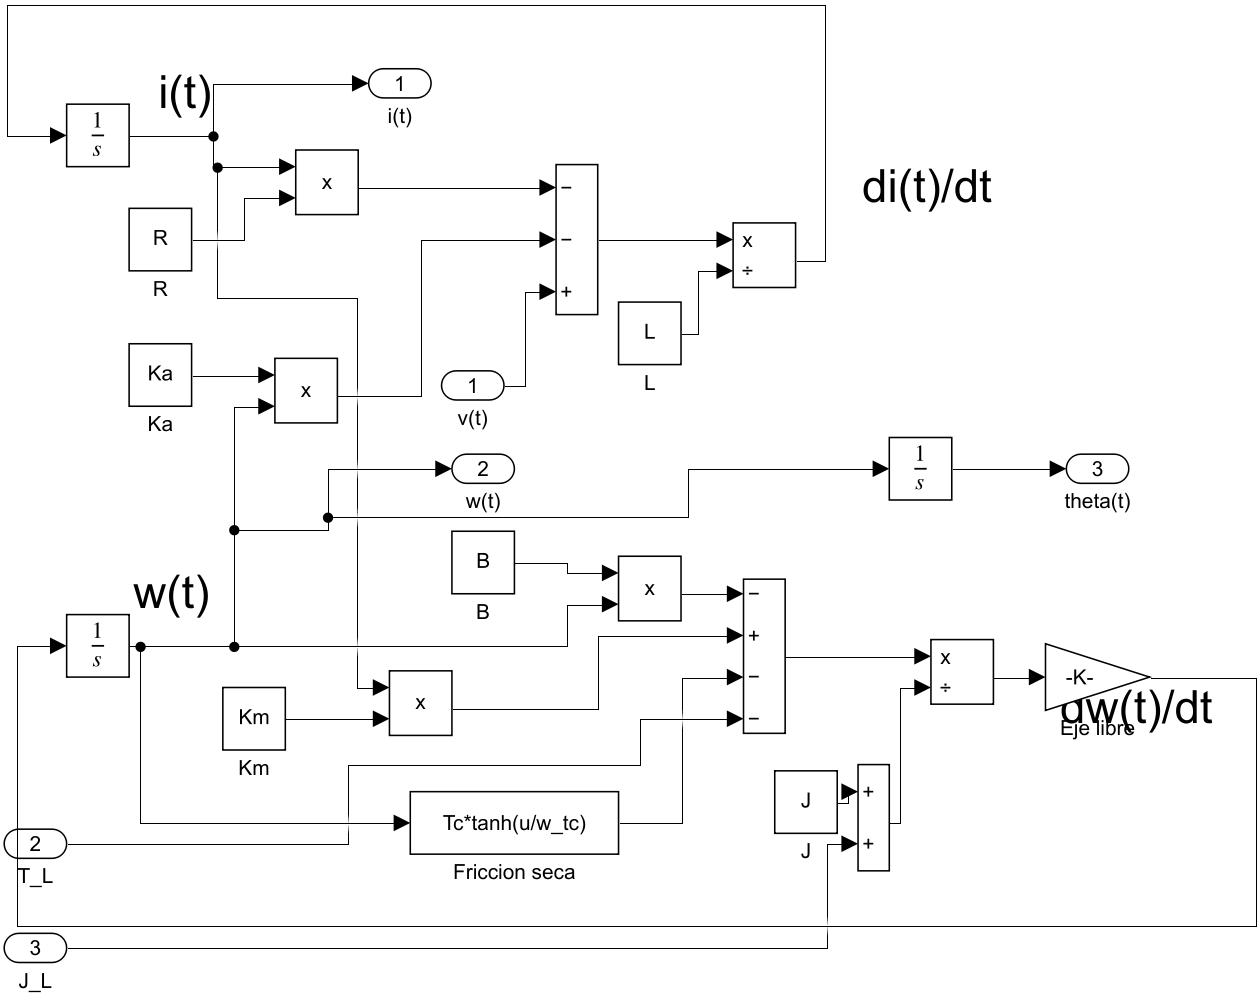
\includegraphics[width=0.75\textwidth]{figuras/control_corriente/simulink_motor_dc.png}
\caption{Subsistema \emph{Motor DC} de la copia, con las entradas $T_L$ y $J_L$.}
\label{fig:cc_sim_motor}
\end{figure}

\subsection{Uso en MATLAB}
\label{sec:cc_uso}
\begin{center}
\begin{tabular}{p{0.32\textwidth}p{0.60\textwidth}}\toprule
Archivo & Función\\\midrule
\code{Parametros_Control.m} & Lee los parámetros medidos de \code{Parametros_Motor_FFB.m}, calcula $K_p$ y $K_i$, muestra los márgenes y arma el comando de prueba\\
\code{Control_Corriente_FFB.slx} & Modelo del lazo\\
\code{Verificar_Control.m} & Ejecuta los casos de la Subsección~\ref{sec:cc_resultados} y mide tiempo de llegada y error\\
\code{Estabilidad_Control.m} & Márgenes, Nyquist, lugar de raíces, robustez y comprobación del margen de ganancia en Simulink\\
\code{Figuras_Control.m} & Valida el procedimiento con el ejemplo del apunte y genera las figuras de respuesta y los diagramas\\
\code{Control_Corriente_775.m} & Simulación independiente, sin Simulink, para contrastar resultados\\
\code{Crear_Modelo_Control.m} & Genera el modelo copiando el bloque \emph{Motor DC}\\\bottomrule
\end{tabular}
\end{center}
Se usan MATLAB R2021a, Simulink y Control System Toolbox (\code{tf}, \code{c2d}, \code{pid}, \code{margin}, \code{stepinfo}, \code{rlocus} y \code{freqresp}) \cite{mathworks_control}. El cálculo central es:
\begin{verbatim}
fc  = 1000;  wc = 2*pi*fc;     % cruce: fs/20
tau_e = L/R;                   % polo que cancela el cero del PI (ec. 7.68)
Ki  = wc*R;                    % ec. 7.71, con kPWM = 1
Kp  = tau_e*Ki;
Lz  = pid(Kp,Ki,0,0,Ts) * c2d(tf(1,[L R]),Ts,'zoh') / tf('z',Ts);
[Gm,Pm] = margin(Lz);          % con un periodo de retardo
\end{verbatim}

El procedimiento de trabajo es:
\begin{enumerate}
\item Correr \code{Parametros_Control}. Para el otro eje, definir antes \code{eje = 'PITCH'}.
\item Abrir y simular \code{Control_Corriente_FFB}.
\item Modificar en el espacio de trabajo la variable a estudiar y volver a simular: \code{Kp}, \code{Ki}, \code{I_FS}, \code{cmd_ws} (comando), \code{eje_trabado}, \code{usar_conmutado}, \code{t_perdido}, \code{ruido_A}, \code{J_eje} o \code{tl_ws} (torque externo en el eje de salida).
\item Correr \code{Verificar_Control} para evaluar el conjunto de casos.
\end{enumerate}
Cuando cambie un parámetro medido del motor, basta con actualizar \code{Parametros_Motor_FFB.m} y repetir los pasos 1 y 4.

\textbf{Paso de integración.} El paso máximo es $T_s/50$, con tolerancia relativa $10^{-6}$. Con $T_s/10$ y $10^{-4}$ aparecieron oscilaciones de hasta 0.4 A que desaparecen al reducir el paso: se trata de un error numérico, no del control, atribuido a que el método de paso variable omite conmutaciones.

\subsection{Resultados}
\label{sec:cc_resultados}
Se aplican escalones de plena escala, comandos chicos ($\pm 0.05$) y 20 comandos al azar, uno cada 2 ms. El \emph{tiempo de llegada} es el que tarda la corriente media en quedar a menos del 5\% del salto (o 0.15 A, si es mayor), en el peor de los saltos. El \emph{error final} es la diferencia entre la corriente y la referencia justo antes del comando siguiente, en el peor caso.

\begin{center}
\begin{tabular}{lcc}\toprule
Caso (roll, $I_{FS} = 5$ A salvo indicación) & Tiempo de llegada & Error final\\\midrule
Rotor trabado, PWM conmutado & 0.27 ms & 0.032 A\\
Rotor trabado, tensión promediada & 0.39 ms & 0.036 A\\
Rotor libre & 0.27 ms & 0.060 A\\
Rotor libre, $J_{eje} = 0.01$ kg$\cdot$m$^2$ (supuesta) & 0.27 ms & 0.035 A\\
Ídem, con torque externo de $\pm 1.5$ N$\cdot$m & 0.27 ms & 0.036 A\\
$I_{FS} = 10$ A & 0.46 ms & 0.043 A\\
$I_{FS} = 10$ A, sin anti-windup & 1.33 ms & 0.347 A\\
$R$ del motor 30\% mayor & 0.62 ms & 0.064 A\\
$L$ 30\% menor / mayor & 0.59 / 0.85 ms & 0.077 / 0.068 A\\
Driver que pierde 1.5 $\mu$s por pulso (supuesto) & 0.92 ms & 0.049 A\\
Muestra sin desfasar & 0.28 ms & 0.061 A\\
$f_c = 500$ Hz & 0.77 ms & 0.036 A\\\bottomrule
\end{tabular}
\end{center}
Salvo sin anti-windup, en todos los casos la corriente llega antes de 1 ms, la mitad del tiempo disponible. En los casos con $R$ y $L$ alteradas se cambia solo la planta: el controlador conserva las ganancias nominales.

\textbf{Límite físico.} El salto más exigente no puede ser más rápido que la respuesta a tensión máxima. Para pasar de $-I_m$ a $+I_m$ con el rotor trabado,
\begin{equation}
t_{min} = \tau_e \ln\frac{I_{max} + I_m}{I_{max} - I_m},\qquad I_{max} = \frac{V_{max}}{R} = 23.8\ \text{A},
\label{eq:cc_tmin}
\end{equation}
que da 0.21 ms para $I_m = 4.31$ A y 0.44 ms para 8.63 A. El requisito de 2 ms es, entonces, alcanzable con este motor y esta alimentación.

\textbf{Lectura de la Figura~\ref{fig:cc_escalones}.} El panel superior muestra que la corriente sigue a la referencia en los escalones grandes, chicos y al azar. En el central, la tensión pedida satura a 20.7 V solo en los saltos grandes, y en régimen se mantiene en unos 4 V. En el inferior se ve que el torque electromagnético sigue a la corriente sin otro retardo.

\begin{figure}[H]
\centering
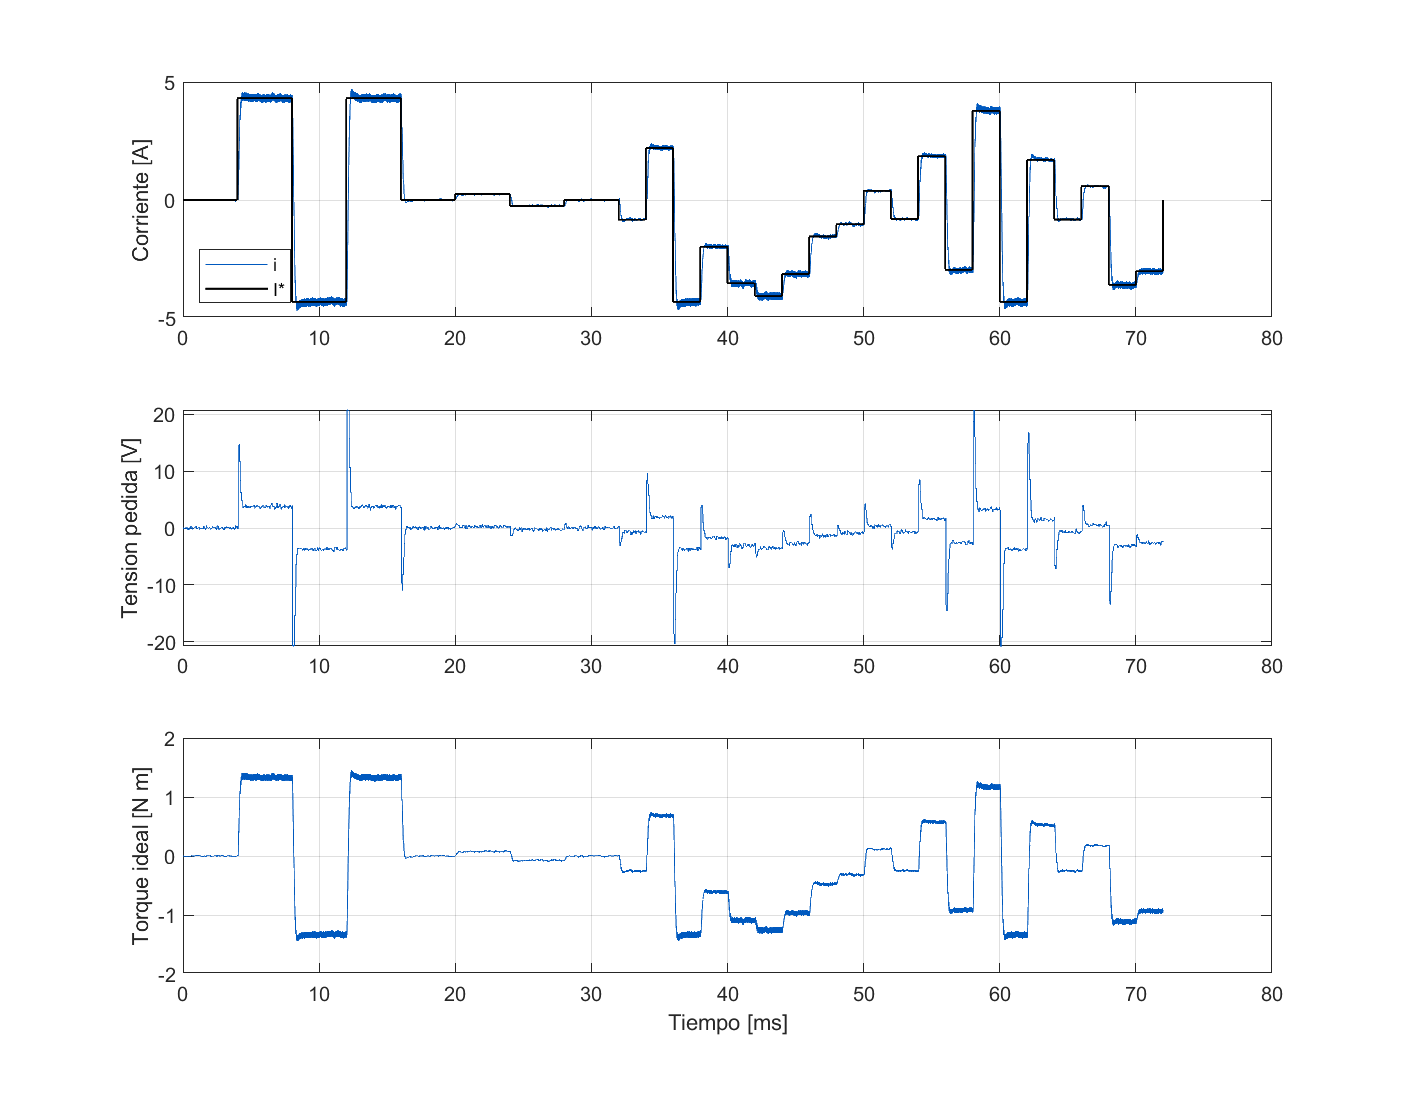
\includegraphics[width=0.9\textwidth]{figuras/control_corriente/escalones.png}
\caption{Respuesta simulada del lazo de roll con rotor trabado y PWM conmutado: corriente, tensión pedida y torque ideal en el eje.}
\label{fig:cc_escalones}
\end{figure}

\textbf{Lectura de la Figura~\ref{fig:cc_detalle}.} En el salto de $-4.31$ a $+4.31$ A, durante el primer período la corriente no cambia: es el retardo de cálculo. Luego sube con la pendiente que permite la alimentación y se establece. Los puntos son las muestras del conversor, que siguen el valor medio del rizado.

\begin{figure}[H]
\centering
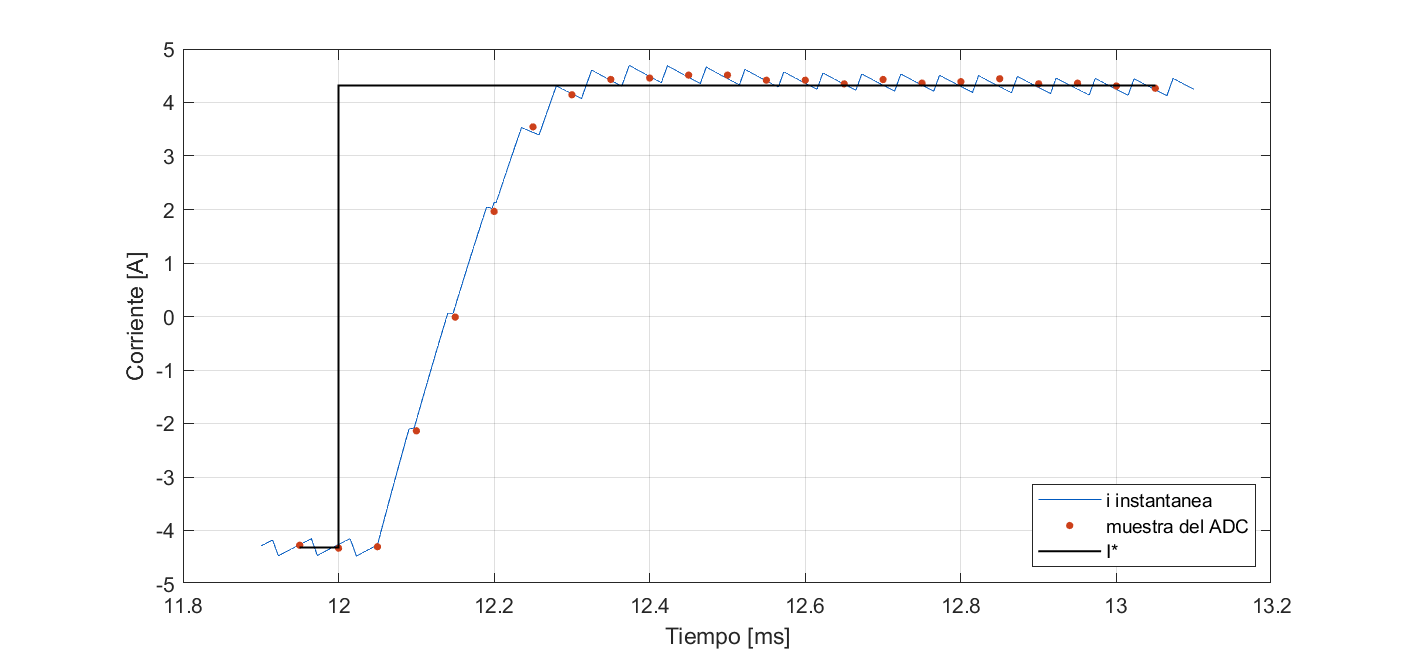
\includegraphics[width=0.85\textwidth]{figuras/control_corriente/detalle.png}
\caption{Detalle de un salto de $-4.31$ a $+4.31$ A: corriente instantánea con rizado y muestras del conversor.}
\label{fig:cc_detalle}
\end{figure}

\textbf{Lectura de la Figura~\ref{fig:cc_carga}.} Con el rotor libre y una inercia supuesta de 0.01 kg$\cdot$m$^2$ en el eje, se aplica un torque externo de 1.5 N$\cdot$m a los 20 ms y se invierte a los 50 ms. El eje se acelera hasta $-4.3$ rad/s, pero la corriente sigue a la referencia como con el rotor trabado: la fuerza pedida no depende de cómo se mueva el eje. En los intervalos en que la corriente y la velocidad tienen signos opuestos, el motor absorbe energía mecánica; parte puede volver hacia la fuente, efecto que el modelo no incluye.

\begin{figure}[H]
\centering
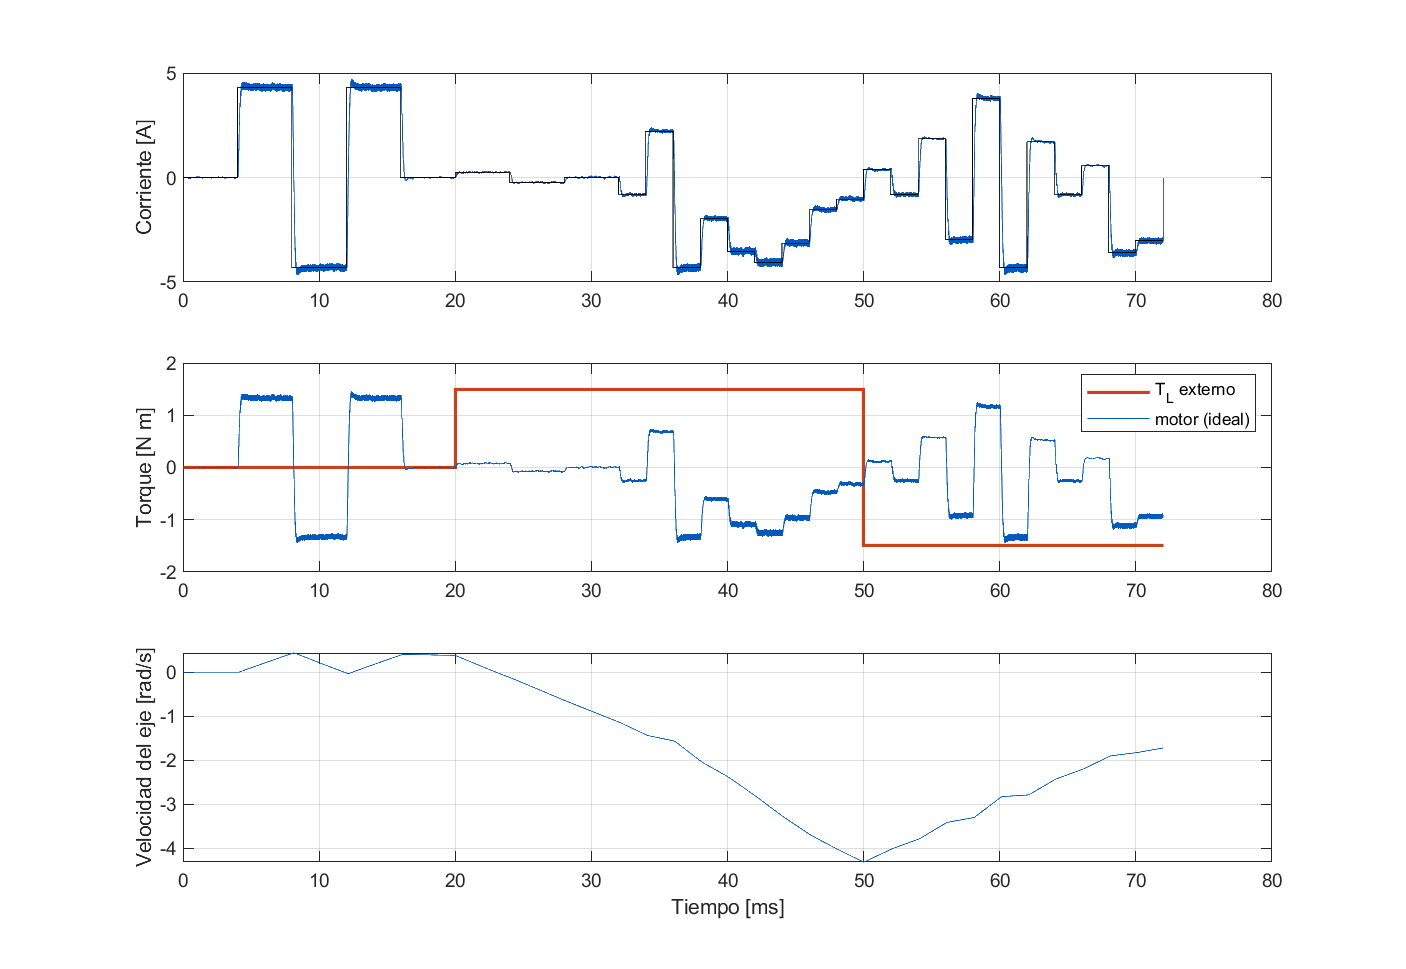
\includegraphics[width=0.9\textwidth]{figuras/control_corriente/carga.png}
\caption{Lazo de corriente con torque externo en el eje de salida.}
\label{fig:cc_carga}
\end{figure}

\subsubsection{Verificaciones del modelo}
\begin{itemize}
\item \textbf{Equivalencia.} Con $T_L = 0$ y $J_L = 0$, la copia con las entradas nuevas da la misma corriente y la misma velocidad que sin ellas: la diferencia es nula.
\item \textbf{Torque externo.} Con $I^* = 0$, $T_{eje} = -1$ N$\cdot$m y $J_{eje} = 0.01$ kg$\cdot$m$^2$, la velocidad del motor a los 0.1 s es 109.95 rad/s. El cálculo a mano sin rozamiento viscoso, $(1/N - \tau_c)\,t/(J + J_L)$, da 110.40 rad/s.
\item \textbf{Contraste.} El script independiente, con un integrador y una prueba distintos, da resultados concordantes: con $I_{FS} = 10$ A, 0.50 ms, frente a 0.46 ms de Simulink.
\end{itemize}

\subsection{Corriente y fuerza en la mano}
\label{sec:cc_fuerza}
Que la corriente llegue a tiempo asegura el torque electromagnético, no la fuerza en el mando. Entre ambos quedan el rozamiento, la inercia reflejada, el juego y el rendimiento de la reductora, que el lazo de corriente no mide ni corrige. Vistos en el eje de roll, el rozamiento de despegue del motor ($8.8\times10^{-3}$ N$\cdot$m) equivale a 0.12 N$\cdot$m y su inercia, a $1.6\times10^{-3}$ kg$\cdot$m$^2$. Por eso los efectos pequeños pueden no percibirse aunque la corriente sea la pedida. Este efecto se evaluará con la reductora montada.

\subsection{Limitaciones y próximos pasos}
\label{sec:cc_pasos}
El modelo no incluye la regeneración hacia la fuente, la caída real del BTS7960 ni su comportamiento con pulsos muy cortos, la variación de temperatura durante el ensayo, ni el juego y el rendimiento de la reductora.
\begin{enumerate}
\item Medir el ruido del ACS712 con el divisor y sin corriente, y reemplazar el valor supuesto.
\item Definir la protección de la alimentación ante regeneración, el corte por sobrecorriente por hardware y el limitador $I^2t$.
\item Implementar el algoritmo en el firmware: PWM centrado de 20 kHz, muestra sincronizada y desfasada, PI con recálculo y una prueba en C++ que compare su salida con la de MATLAB.
\item Ensayar con rotor trabado y 1 a 2 A, y comparar la corriente medida con la simulada. Luego, con el eje libre y movido a mano.
\item Con la reductora, caracterizar ambos ejes (inercia, rozamiento, relación y rendimiento), cargar $J_{eje}$ en el modelo y ajustar $I_{FS}$.
\item Repetir el cálculo para pitch con sus parámetros medidos.
\end{enumerate}
